\documentclass{beamer}

\mode<presentation>
{
  \usetheme{default}
  \usecolortheme{whale}
}

\newenvironment{changemargin}[2]{% 
  \begin{list}{}{% 
    \setlength{\topsep}{0pt}% 
    \setlength{\leftmargin}{#1}% 
    \setlength{\rightmargin}{#2}% 
    \setlength{\listparindent}{\parindent}% 
    \setlength{\itemindent}{\parindent}% 
    \setlength{\parsep}{\parskip}% 
  }% 
  \item[]}{\end{list}} 

\usepackage[utf8x]{inputenc}
%\usepackage{default}
\usepackage{amsmath}
\usepackage{amsfonts}
\usepackage{amssymb}
\usepackage{graphicx}
\usepackage{epstopdf}
\usepackage{textpos}
\usepackage[]{units}

\setbeamertemplate{footline}[frame number]
\setbeamertemplate{navigation symbols}{} %no nav symbols

\addtobeamertemplate{frametitle}{}{%
\begin{textblock*}{100mm}(1.0\textwidth,-1cm)
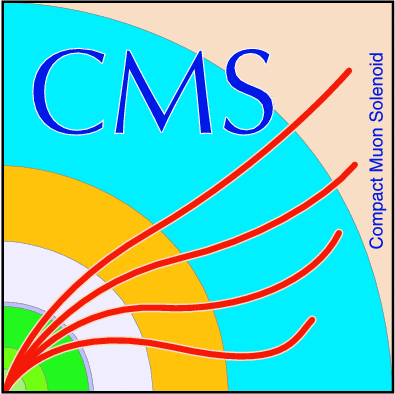
\includegraphics[height=1cm,width=1cm]{cms_logo.png}
\end{textblock*}}

\title[Ph.D. Defense]
{Fast GPU Nearest Neighbors search algorithms for the CMS experiment at LHC}

\author[Alessandro Degano] 
{Alessandro Degano}

\institute[Università degli Studi di Torino]

\date[29/06/2016] % (optional, should be abbreviation of conference name)
{Torino 29/06/2016}

\subject{Computing Science}

\begin{document}
\maketitle

\section{HL-LHC}

\begin{frame}{Outline}
	\tableofcontents
\end{frame}

\begin{frame}{High Luminosity LHC}
\begin{figure}
\begin{center}
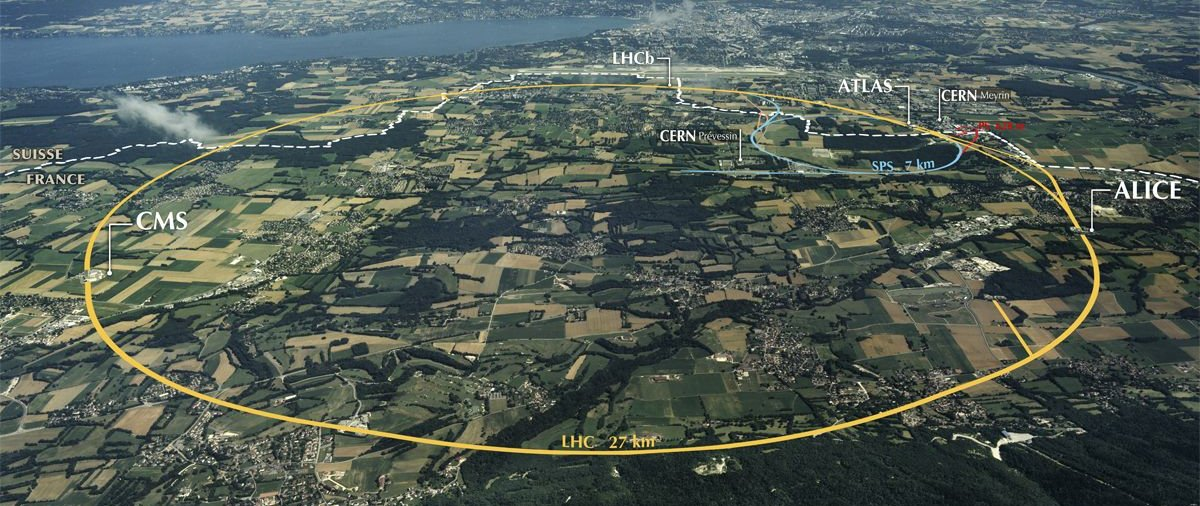
\includegraphics[scale=0.25]{images/lhc.jpg}
\end{center}
\end{figure}

\begin{tabular}{l c c}
 & \textbf{2016 conditions} & \textbf{2025 conditions} \\
\hspace{1cm}
Luminosity & 5 nb/s &  50 nb/s \\
\hspace{1cm}
Pileup & 50 & 140(200) \\
\end{tabular}

\end{frame}

\begin{frame}{The Compact Muon Solenoid}
\begin{figure}
\begin{center}
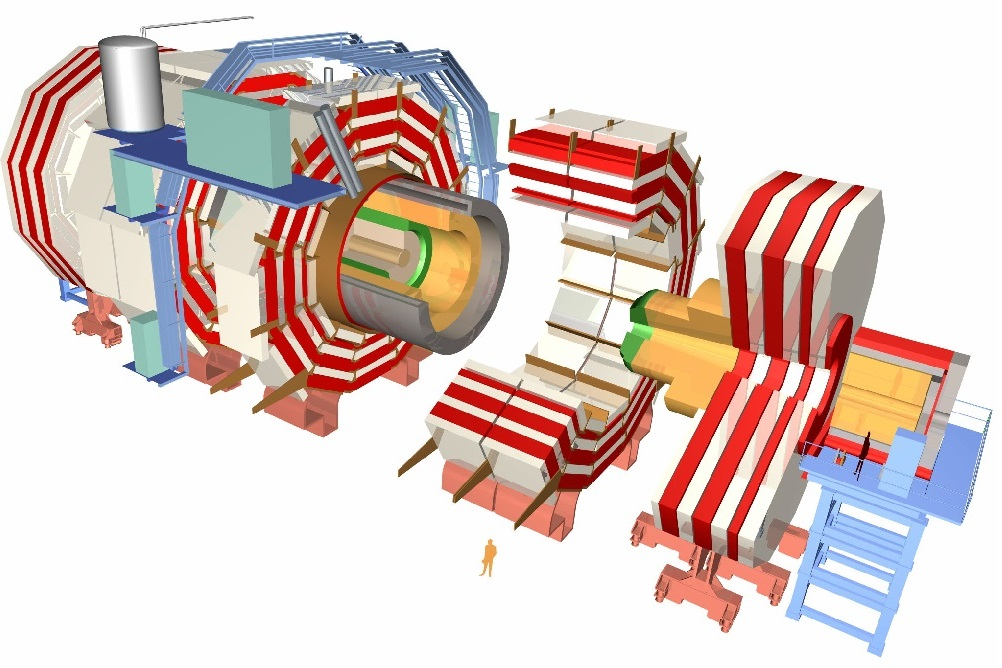
\includegraphics[scale=0.8]{images/cms.jpg}
\end{center}
\end{figure}
\begin{center}
Sub-detectors:
\begin{itemize}
\item Tracker
\item EM Calorimeter
\item Hadronic Calorimeter
\item Solenoid
\item Muon Chambers + Steel Yoke
\end{itemize}
\end{center}
\end{frame}

\begin{frame}{CMS Phase-II upgrades}
Several parts will need substitution/upgrade:
\begin{itemize}
\item Full tracker substitution with 4x granularity
\item Calorimeters Endcaps with higher granularity
\item Muon Endcaps with additional GEMs and RPC
\item Level 1 trigger to comply with 750kHz rate
\item High Level Trigger farm with 12x current computational power
\end{itemize}
\end{frame}

\begin{frame}{High Granularity Calorimeter}
The EndCaps will be substituted by a sampling calorimeter.
\begin{figure}
\begin{center}
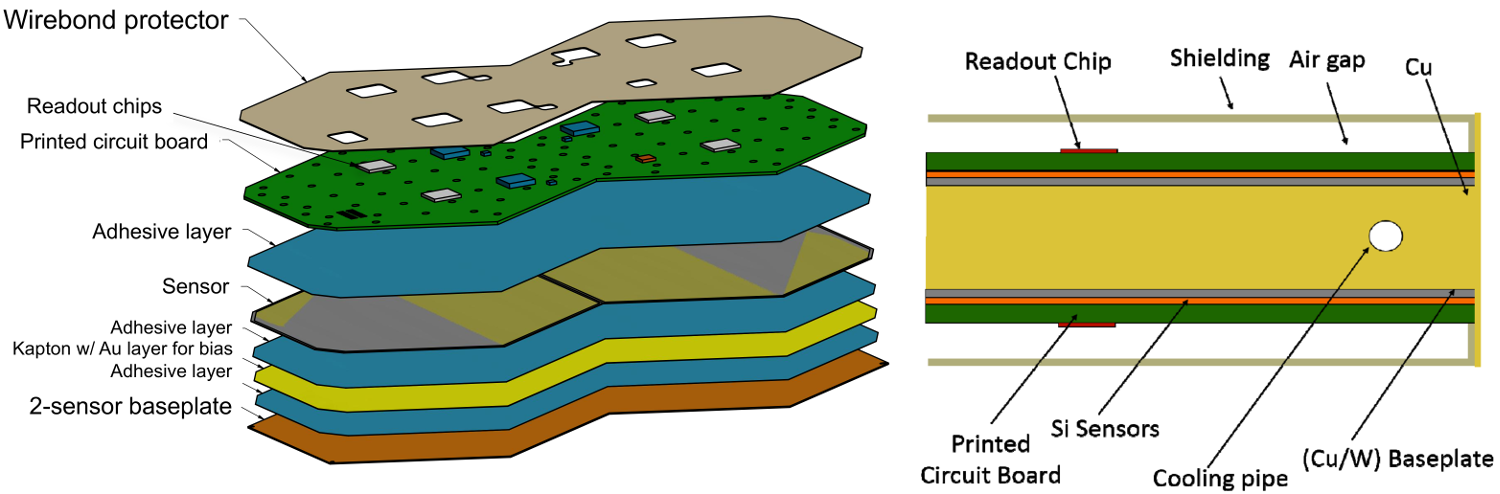
\includegraphics[scale=2.0]{images/hgcalMod.png}
\end{center}
\end{figure}
Active material:
\begin{itemize}
\item 0.53 $cm^2$ or 1.05 $cm^2$ silicon pad
\end{itemize}
Passive material:
\begin{itemize}
\item Copper plate Tungsten coated
\end{itemize}

\end{frame}

\begin{frame}{HGCAL ECAL EndCaps}
\begin{figure}
\begin{center}
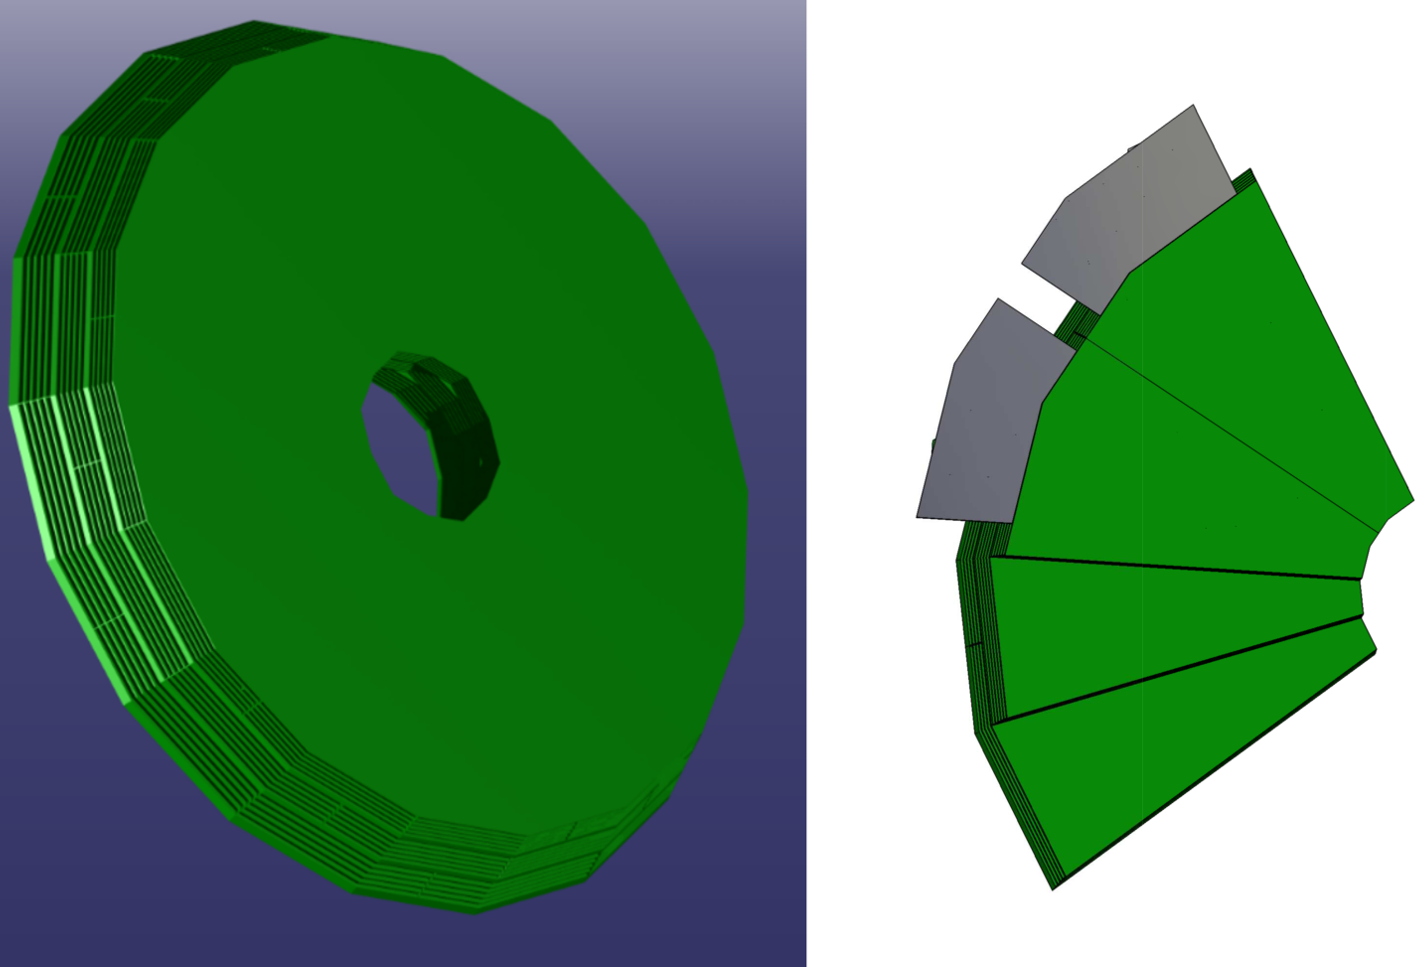
\includegraphics[scale=1.8]{images/hgcalStruct.png}
\end{center}
\end{figure}
\begin{center}
22000 modules, 28 layers\\
Total radiation lenght: 26 $X_0$\\
\vspace{0.5cm}
Readout 4.3 Million Channels
\end{center}
\end{frame}

\begin{frame}{HGCAL shower development}
\begin{center}
\begin{figure}
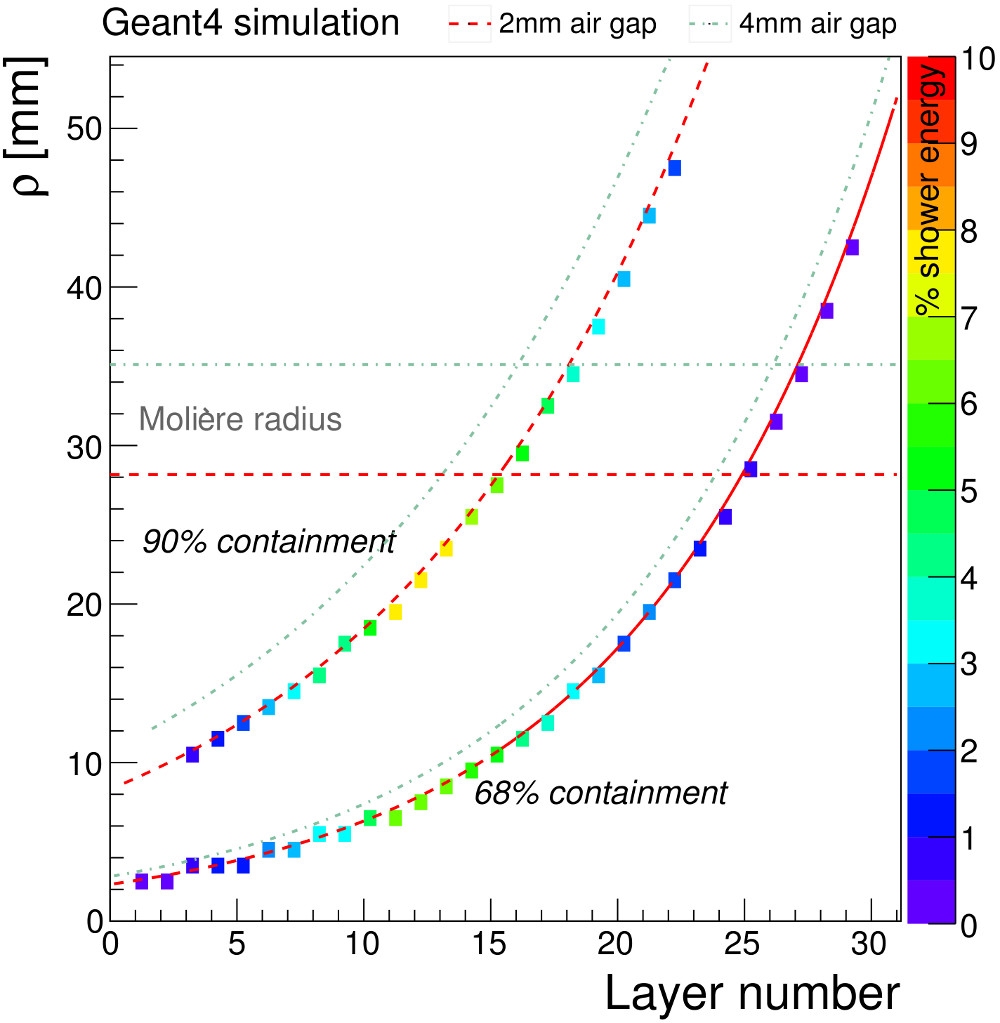
\includegraphics[scale=2]{images/moliereHgcal.png}
\end{figure}
In the farthest layer the shower has radius of 6.0 cm.\\
\vspace{0.5cm}
The maximum number of Recorded Hits (rechits) for 95 $\%$ containment is $\simeq$ 273
\end{center}
\end{frame}

\begin{frame}{Clusterization}
\begin{center}
An EM shower is reconstructed by the \textit{hits}\\
left on the layers of the calorimeter
\begin{figure}
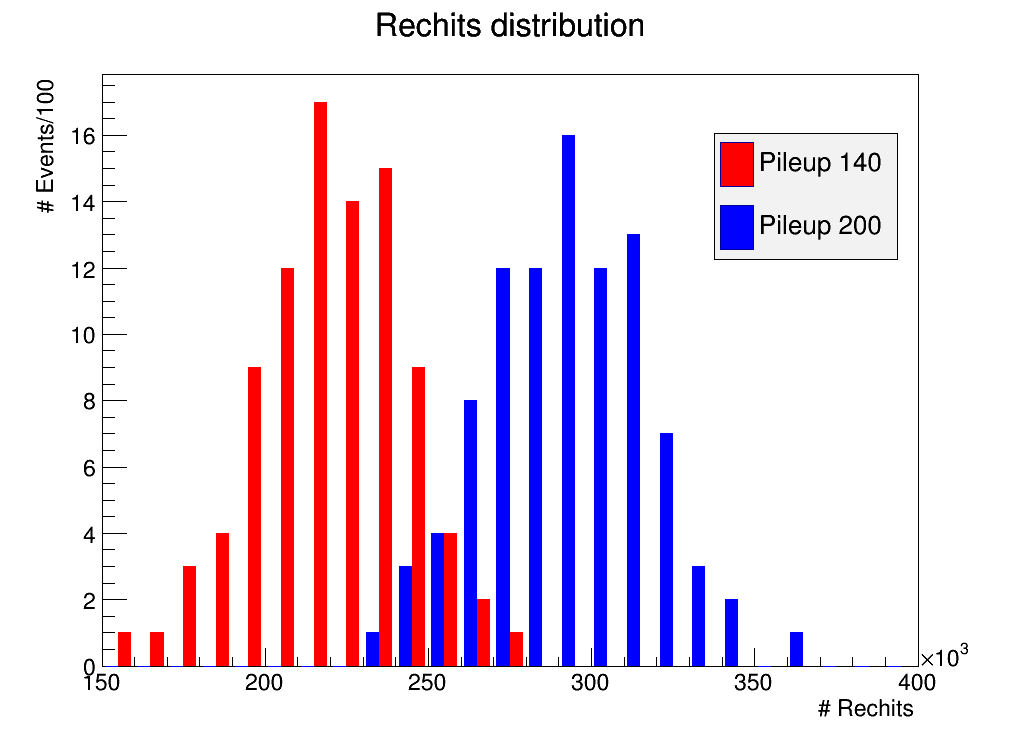
\includegraphics[scale=0.25]{images/rechitsHisto.png}
\end{figure}
\end{center}
\end{frame}

\section{Computing}

\begin{frame}{Moore's law}
\begin{center}
\textit{``The number of transistors on a chip doubles every 24 months''}
\begin{figure}
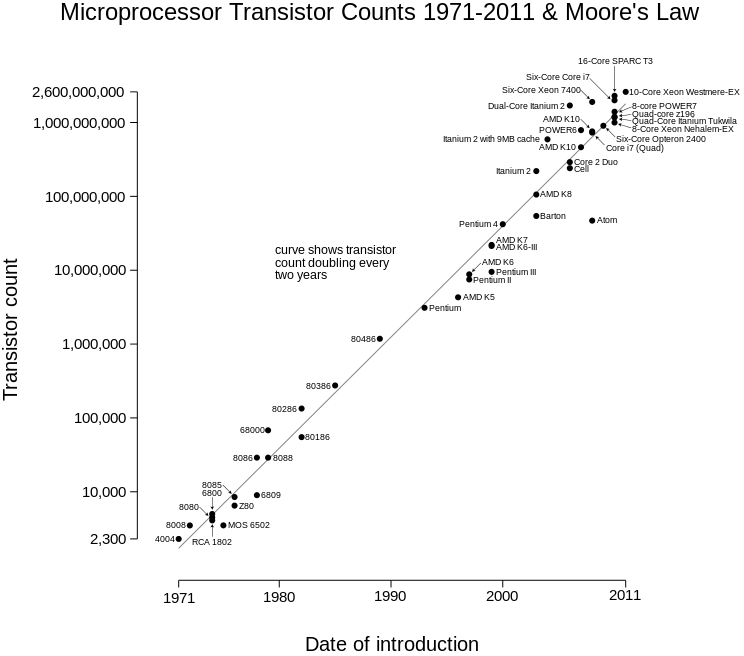
\includegraphics[scale=0.25]{images/moores.png}\\
Two main issues:
\begin{itemize}
\item At $\sim$ 7 nm quantum tunneling plays a role
\item How to employ all those tranistors
\end{itemize}
\end{figure}
\end{center}
\end{frame}

\begin{frame}{Parallelization}
Multiple cores in the same processing unit can run independently at the same time
\begin{center}
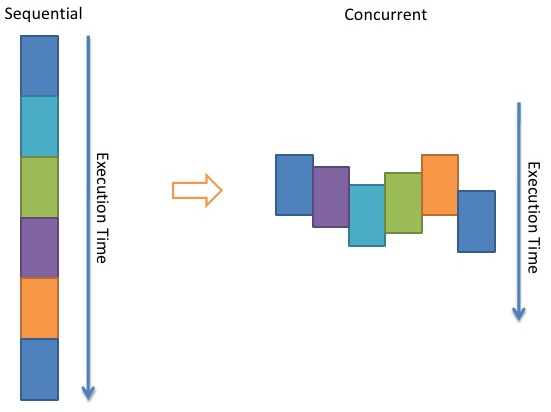
\includegraphics[scale=0.4]{images/parallel.jpg}\\
Does \textbf{$N$} cores makes the parallel execution time \textbf{$1/N^{th}$}\\ of the sequential?
\end{center}
\end{frame}

\begin{frame}{Amdahl's law}
\begin{center}
\begin{equation}
S(p,f) \equiv \dfrac{T_p}{T_s} = \frac{1}{f + \frac{1-f}{p}} \rightarrow \lim_{p\to\infty} S(p,f) = \frac{1}{f}
\end{equation}
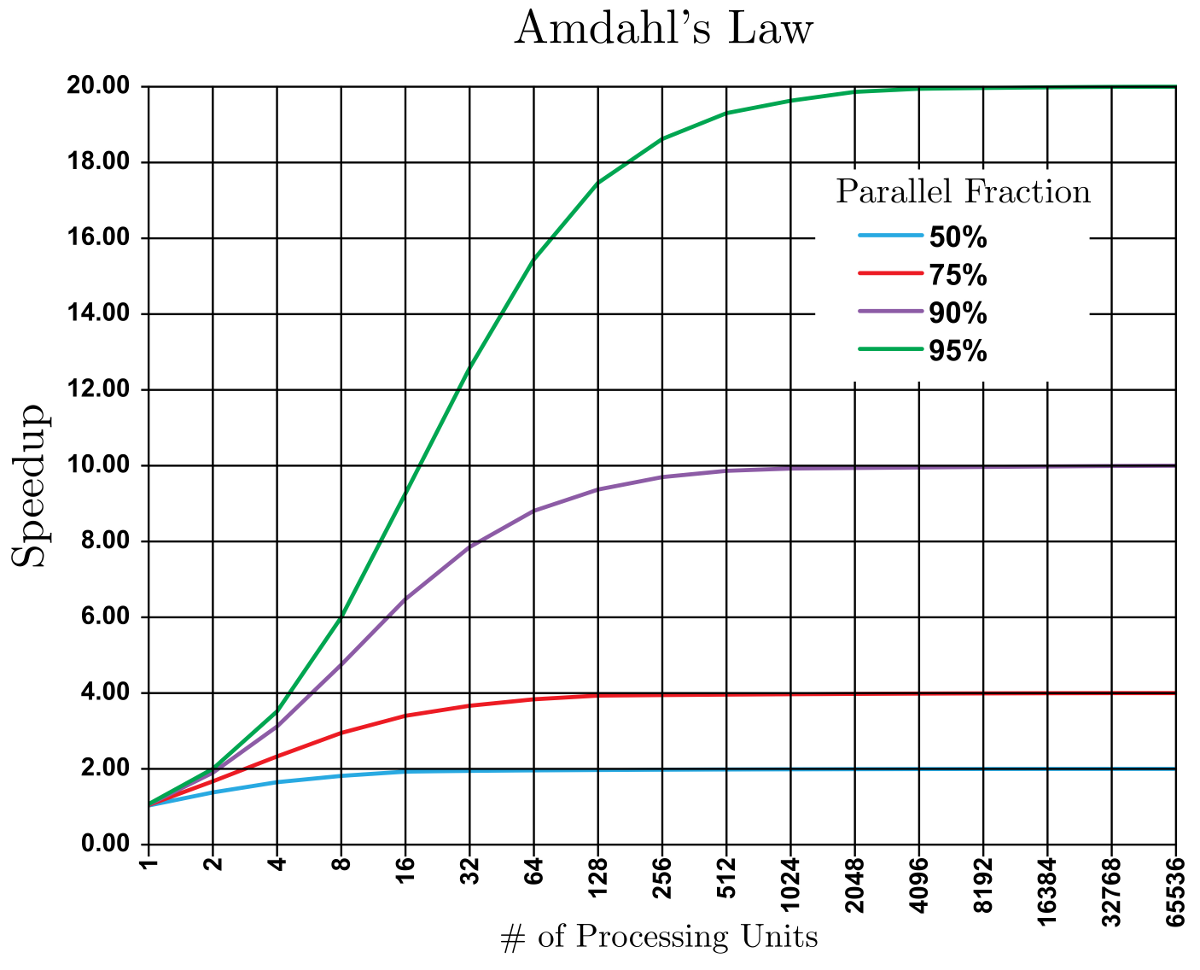
\includegraphics[scale=2.5]{images/amdahl.png}
\end{center}
\end{frame}

\begin{frame}{CPU vs GPU}
\begin{center}
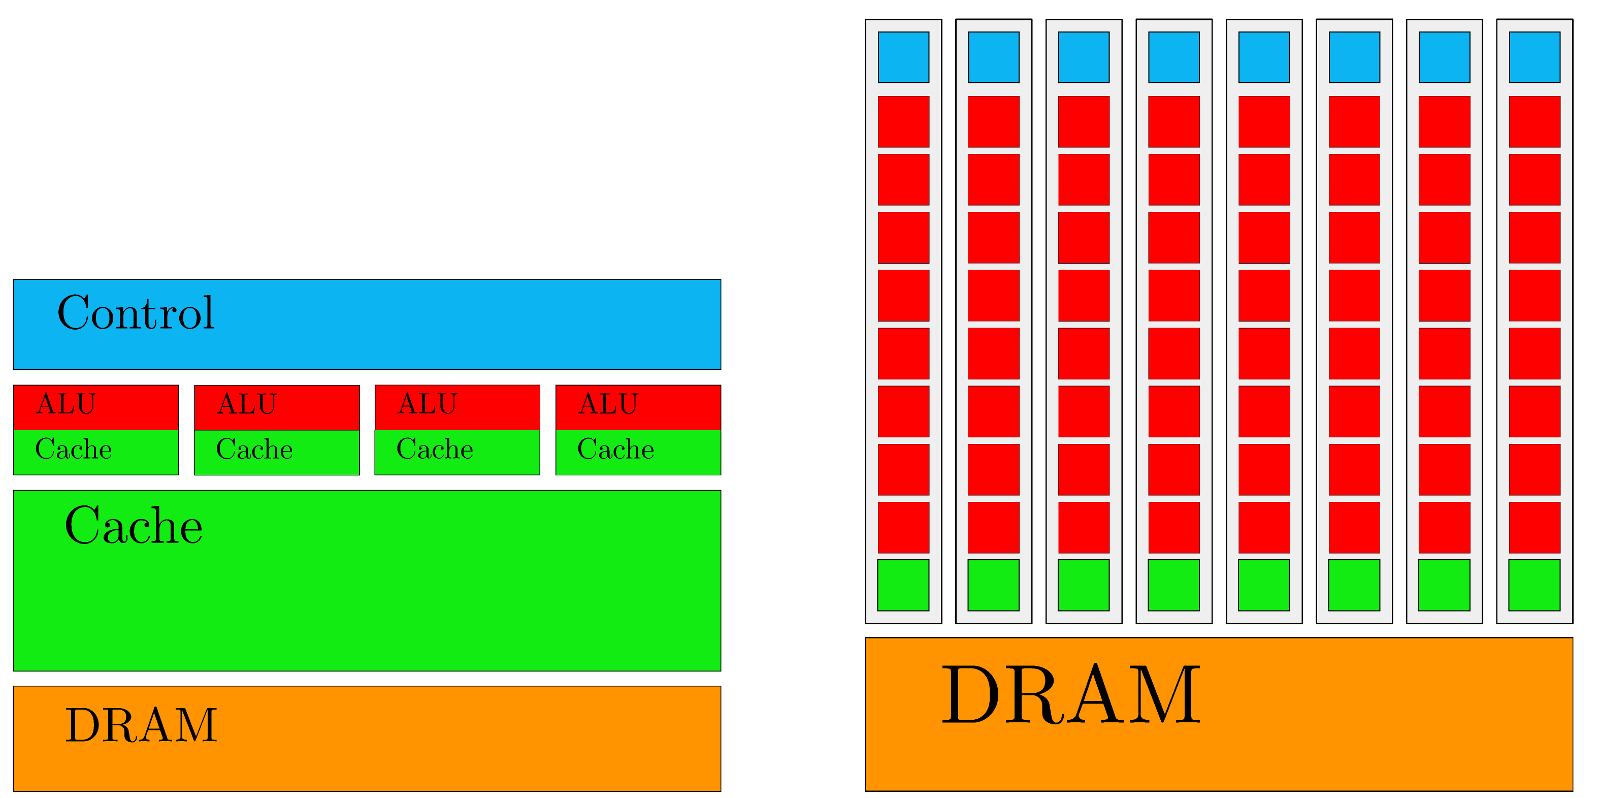
\includegraphics[scale=2]{images/archs.png}
\begin{columns}
\begin{column}{0.5\textwidth}
\hspace{1.6cm} A CPU with 4 cores
\end{column}
\begin{column}{0.5\textwidth}
    A GPU with multiple cores
\end{column}
\end{columns}
\vspace{0.5cm}
The main differences:
\begin{itemize}
\item CPU: Large cache, GPU: small cache
\item CPU: Few cores, GPU: thousand of cores
\end{itemize}
\end{center}
\end{frame}

\begin{frame}{GPU memory hierarchy}
\begin{center}
\begin{table}[h]
\begin{changemargin}{-1cm}{-2cm}
\begin{tabular}{ l | l | l | l | l}
\textbf{Memory} & \textbf{Visibility} & \textbf{Lifetime} & \textbf{Access time} & \textbf{Size (k40)}\\
\hline
Registers & Thread & Thread & Very fast & 90 Bytes \\
Shared mem. & Block & Block & Fast & 48 kBytes \\
Global mem. & Grid & Application & 150 $\times$ slower than SM & 12 GB \\
\end{tabular}
\end{changemargin}
\end{table}
\vspace{2cm}
Manual memory management mandatory and\\ essential for optimization
\end{center}
\end{frame}

\section{Volume KD-tree algorithm}

\begin{frame}{Binary tree}
\begin{center}
Two data-structures best suited for fast search:
\begin{itemize}
\item Hash tables
\item Binary tree
\end{itemize}
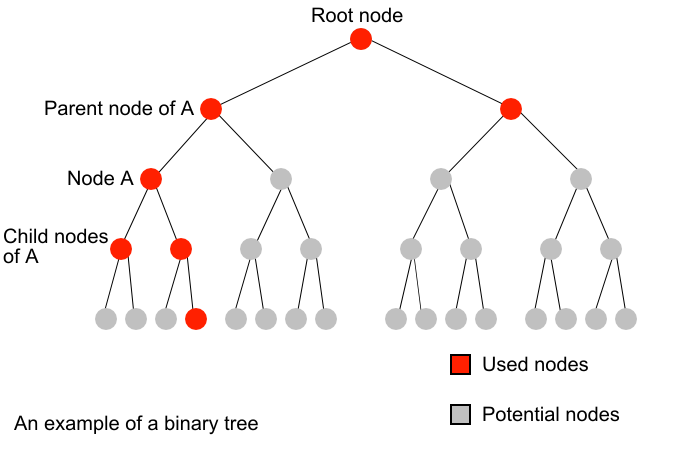
\includegraphics[scale=0.3]{images/binary_tree.png}\\
\end{center}
\end{frame}

\begin{frame}{K-dimensional binary tree}
\begin{center}
\vspace{2cm}
The extension of a binary tree in K dimensions: \textbf{KD-Tree}\\
\vspace{2cm}
The goal:
\begin{itemize}
\item Divide the space in sub-spaces
\item Repeat the division until smallest sub-spaces created
\item Define a relation between the sub-spaces
\end{itemize}
\end{center}
\end{frame}

\begin{frame}{Example: building a 2D tree}
\begin{center}
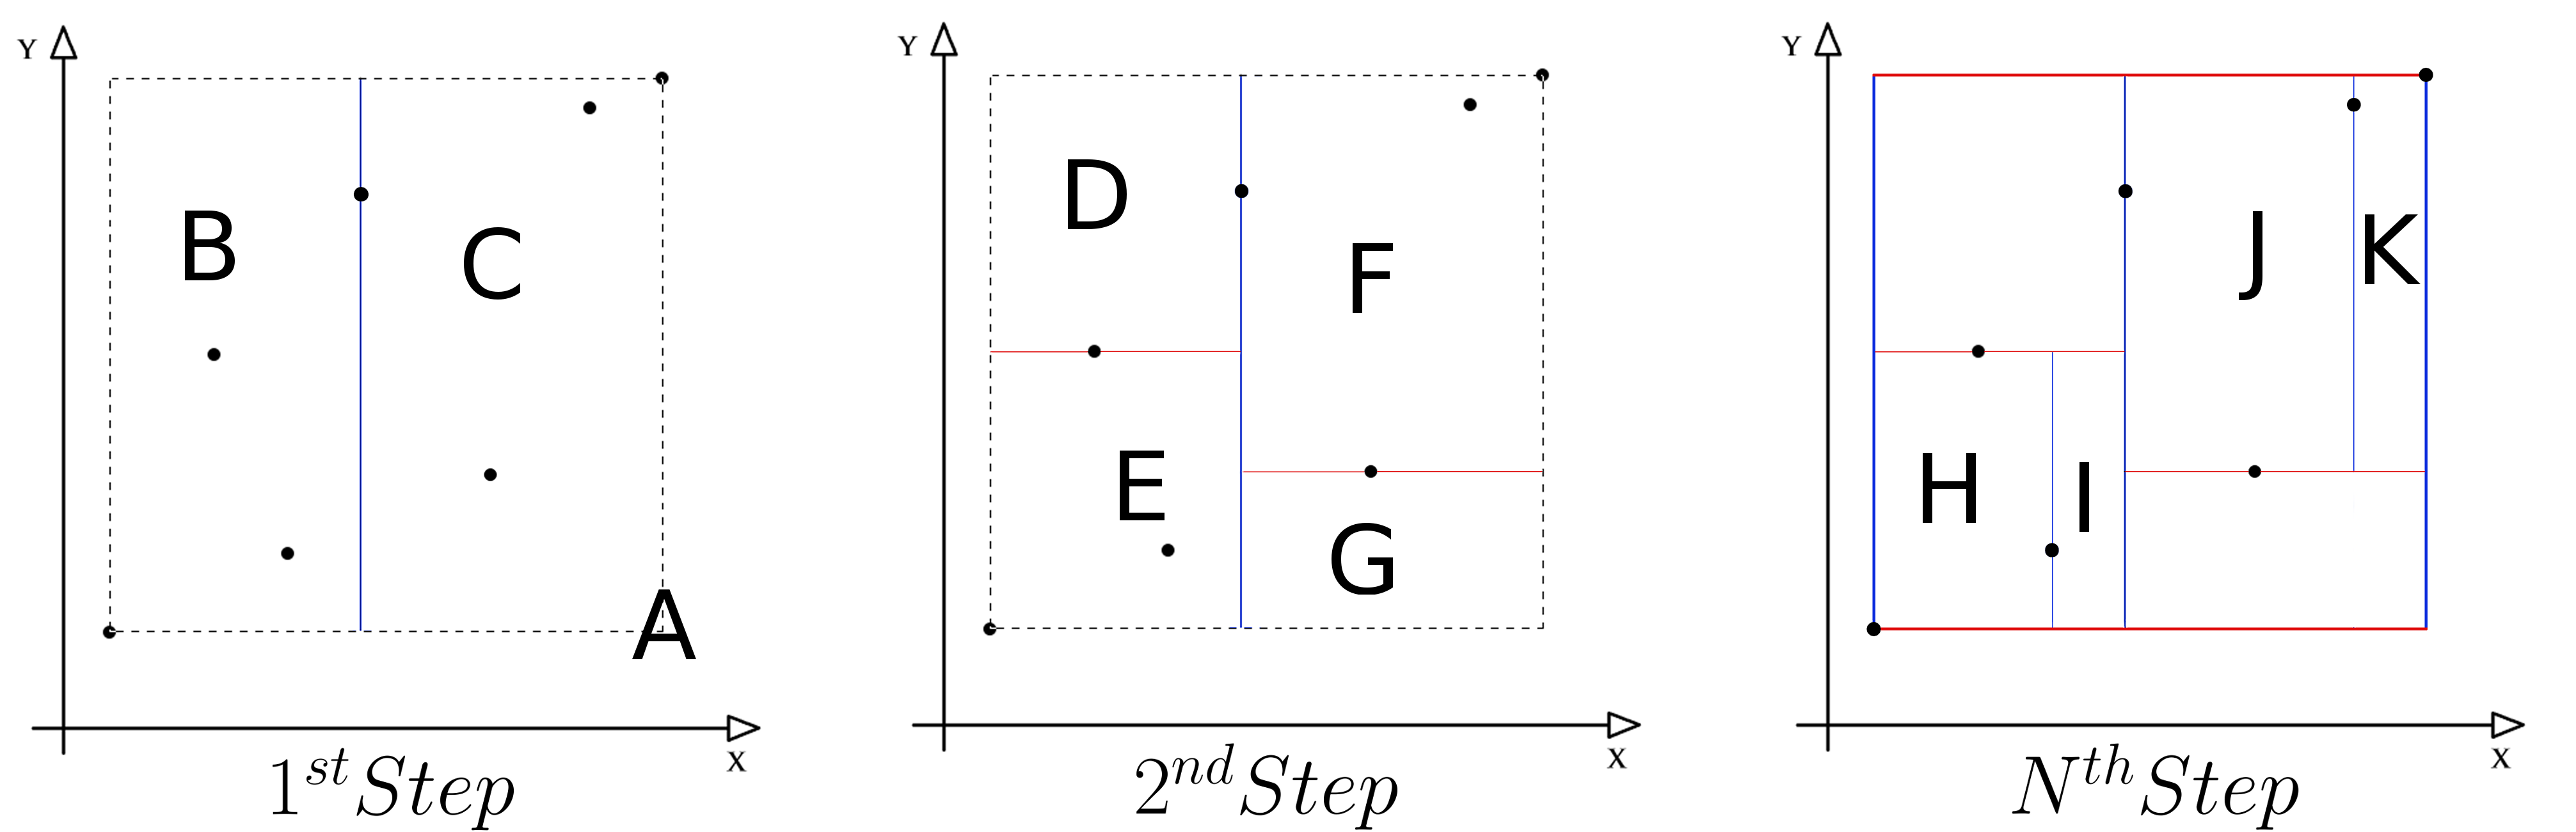
\includegraphics[scale=0.3]{images/scheme_volume_kdtree.png}\\
\vspace{0.5cm}
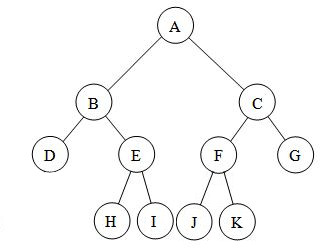
\includegraphics[scale=0.5]{images/binary_tree2.jpg}
\end{center}
\end{frame}

\begin{frame}{Searching an element of the KD-tree}
\begin{changemargin}{-1cm}{-2cm}
\begin{columns}
\begin{column}{0.3\textwidth}
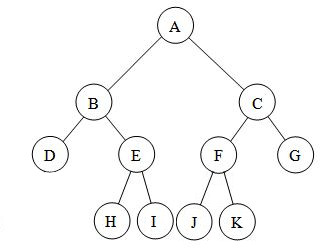
\includegraphics[scale=0.35]{images/binary_tree2.jpg}
\end{column}
\begin{column}{0.7\textwidth}
\begin{center}
Done by recursion:
\begin{itemize}
\item Start from root
\item Is the element in the left or right son?
\item Go in the son containing the element
\item Repeat the last two step
\item Stop at node with no sons (\textit{leaf})
\end{itemize}
\end{center}
\end{column}
\end{columns}
\end{changemargin}
\begin{center}
\vspace{1cm}
At each step half of the sub-tree\\ is discarded from further searching.\\
\vspace{0.5cm}
$\mathcal{O}(\log{} n)$
\end{center}
\end{frame}

\begin{frame}{All Nearest Neighbors search}
\begin{center}
Instead of searching one point search a volume\\
\vspace{0.5cm}
Again by recursion:
\begin{itemize}
\item Is the volume contained in the left or right son\\ \textbf{or intersects them}?
\item Proceed searching the son(s)
\item If an element is inside the volume record it
\item Stop at leaves
\end{itemize}
\vspace{1cm}
Some step does not discard half of the tree\\
\vspace{0.5cm}
$\mathcal{O}(k n ^{1-\dfrac{1}{k}})$
\end{center}
\end{frame}

\begin{frame}{An implementation of the KD-tree}
\begin{center}
For this implementation we save the volumes in the KD-tree\\
\vspace{0.5cm}
Properties:
\begin{itemize}
\item Root: the smallest volume containing all points
\item Right and left nodes: the volumes obtained splitting Root
\item Sum of all leaves volumes = Root
\end{itemize}
\vspace{0.5cm}
Advantage: if the search box fully contains a node all the points in that nodes are Nearest Neighbors, no further search required
\end{center}
\end{frame}

\begin{frame}{GPU parallelization}
\begin{center}
Only All Nearest Neighbors search on GPU.
\vspace{0.5cm}
Requirements:
\begin{itemize}
\item STL container not supported on CUDA
\item Move input data to GPU board
\item Occupy all GPU cores
\item Move output data back to host
\end{itemize}
\end{center}
\vspace{5mm}
Output cannot be dynamically allocated, evaluate size of output:
\begin{center}
$V$ = Total volume \hspace{5mm} $V_s$ = Search box volume
\end{center}
\vspace{0.5cm}
\begin{equation}
NN_{max} = N_{total} \cdot \dfrac{V_f}{V}\cdot 2.0
\end{equation}
\end{frame}

\begin{frame}{Validation and performance}
Generate a data set of $[20000, 350000]$ points in a cube of 100.0 a.u. and search the NN in a cube of 4.0 a.u.\\
\vspace{5mm}
Validation:
\begin{itemize}
\item Compare results with \textit{naive} method, $100\%$ accuracy required
\end{itemize}
\vspace{5mm}
Performance assessment:
\begin{itemize}
\item Measure execution time of tree building vs number of points
\item Measure execution time of sequential ANN
\item Measure execution time of parallel ANN
\item Calculate speedup
\end{itemize}
\end{frame}

\begin{frame}{Building time}
\begin{center}
\begin{changemargin}{-5mm}{-5mm}
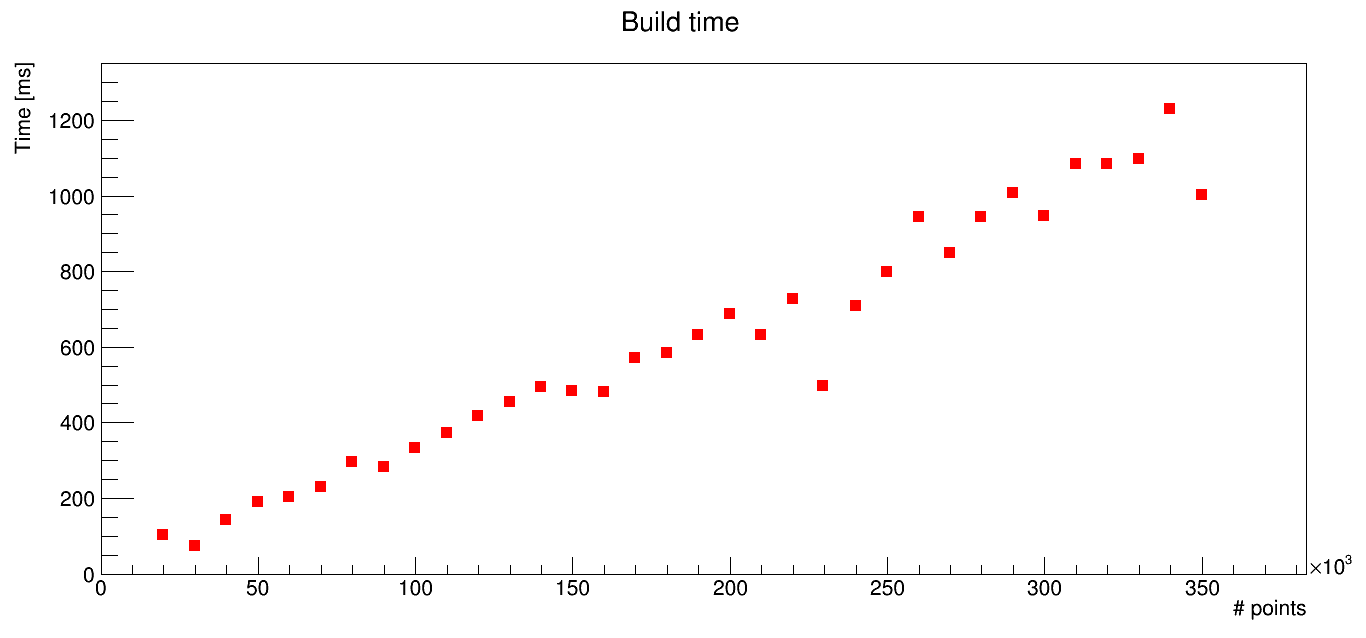
\includegraphics[scale=0.25]{images/volumeBuildTime.png}
\end{changemargin}
\end{center}
\end{frame}

\begin{frame}{ANN search time}
\begin{center}
\begin{changemargin}{-5mm}{-5mm}
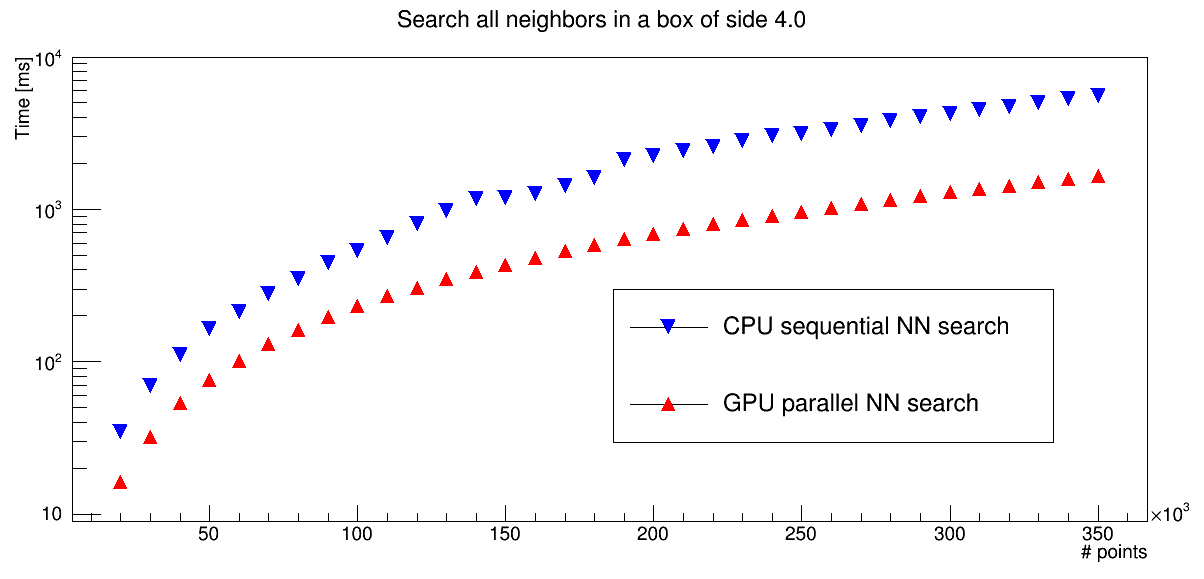
\includegraphics[scale=0.28]{images/volumeKdTree.png}
\end{changemargin}

\begin{table}[h]
\begin{tabular}{ c || r r r r r r r }
Points ($10^{3}$) & 50 & 100 & 150 & 200 & 250 & 300 & 350 \\
\hline
CPU (ms) & 164 & 528 & 1186 & 2234 & 3091 & 4225 & 5501 \\
GPU (ms) & 75 & 223 & 431 & 682 & 954 & 1281 & 1639 \\
\end{tabular}
\end{table}
\end{center}
\end{frame}

\begin{frame}{Speedup}
\begin{center}
\begin{changemargin}{-5mm}{-5mm}
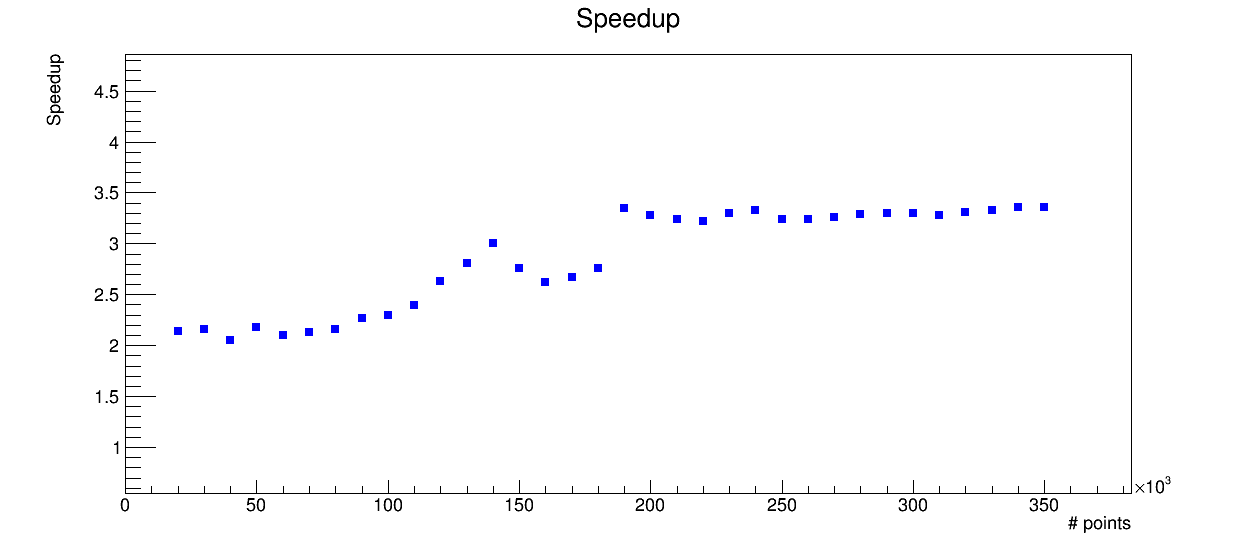
\includegraphics[scale=0.28]{images/volumeKdSpeedup.png}\\
\end{changemargin}
\vspace{5mm}
Speedup between \textbf{$\sim$2} and \textbf{$\sim$3.5}
\end{center}
\end{frame}

\begin{frame}{Algorithm assessment}
Overall disappointing performance:
\begin{itemize}
\item Build time too slow: up to $\sim 100\%$ of search time, \textbf{$1\unit{s}$}
\vspace{3mm}
\item Absolute timings too high: $\sim 5.5\unit{s}$ CPU and $\sim 1.6\unit{s}$ GPU
\vspace{3mm}
\item Speedup too low compared to what Amdahl promises
\end{itemize}
\vspace{5mm}
Two major issues:
\begin{itemize}
\item Node indices are read instead of evaluated
\vspace{3mm}
\item Volumetric nodes bring very little advantage in practice
\end{itemize}
\vspace{10mm}
\begin{small}
Back to the drawing board...
\end{small}
\end{frame}

\section{A better KD-tree}

\begin{frame}{A better KD-tree implementation}
A new implementation learning from the gained experience:
\vspace{5mm}
\begin{enumerate}
\item Abandon the idea of nodes as volumes
\vspace{3mm}
\item Evaluate nodes positions instead of querying
\vspace{3mm}
\item No gaps between leaves $\rightarrow$ LBT
\vspace{3mm}
\item Improve building time
\vspace{3mm}
\item Transform recursion into iteration
\vspace{3mm}
\item Improve data transfer to/from GPU
\end{enumerate}
\end{frame}

\begin{frame}{Improvements I}
\begin{enumerate}
\item [1.] The points of the data set are the nodes of the tree
\end{enumerate}

\begin{enumerate}
\item [2.] Binary tree $\rightarrow$ Children Index:\\ $I_{left} = I_p \cdot 2$ and $I_{right} = I_p \cdot 2 + 1$
\end{enumerate}

\begin{enumerate}
\item [3.] Left Balanced Tree \\
\begin{changemargin}{-3cm}{-2cm}
\begin{center}
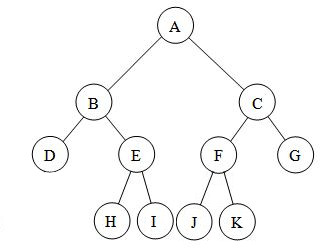
\includegraphics[scale=0.5]{images/binary_tree2.jpg}
$\rightarrow$
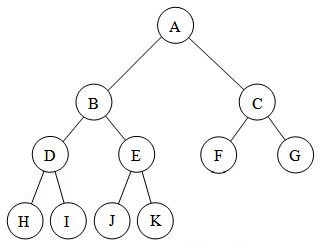
\includegraphics[scale=0.5]{images/binary_tree2_lbt.jpg}
\end{center}
\end{changemargin}
\end{enumerate}
\end{frame}

\begin{frame}{Improvements II}
\vspace{5mm}
\begin{enumerate}
\item [4.] Do not sort all points \texttt{std::nth\_element}
\end{enumerate}
\vspace{5mm}
\begin{enumerate}
\item [5.] Use a queue (LIFO) to store nodes to visit instead of recursion
\end{enumerate}
\vspace{5mm}
\begin{enumerate}
\item [6.] Make the copy to/from the GPU asynchronous with CUDA Streams
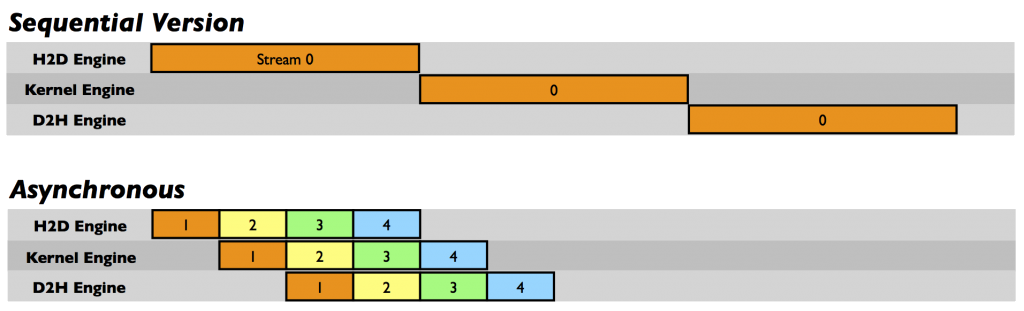
\includegraphics[scale=0.25]{images/cuda_streams.png}
\end{enumerate}

\end{frame}

\begin{frame}{Uniform random distribution performance}
Number of points generated: [20000, 500000]\\
\begin{changemargin}{-2cm}{-2cm}
\begin{center}
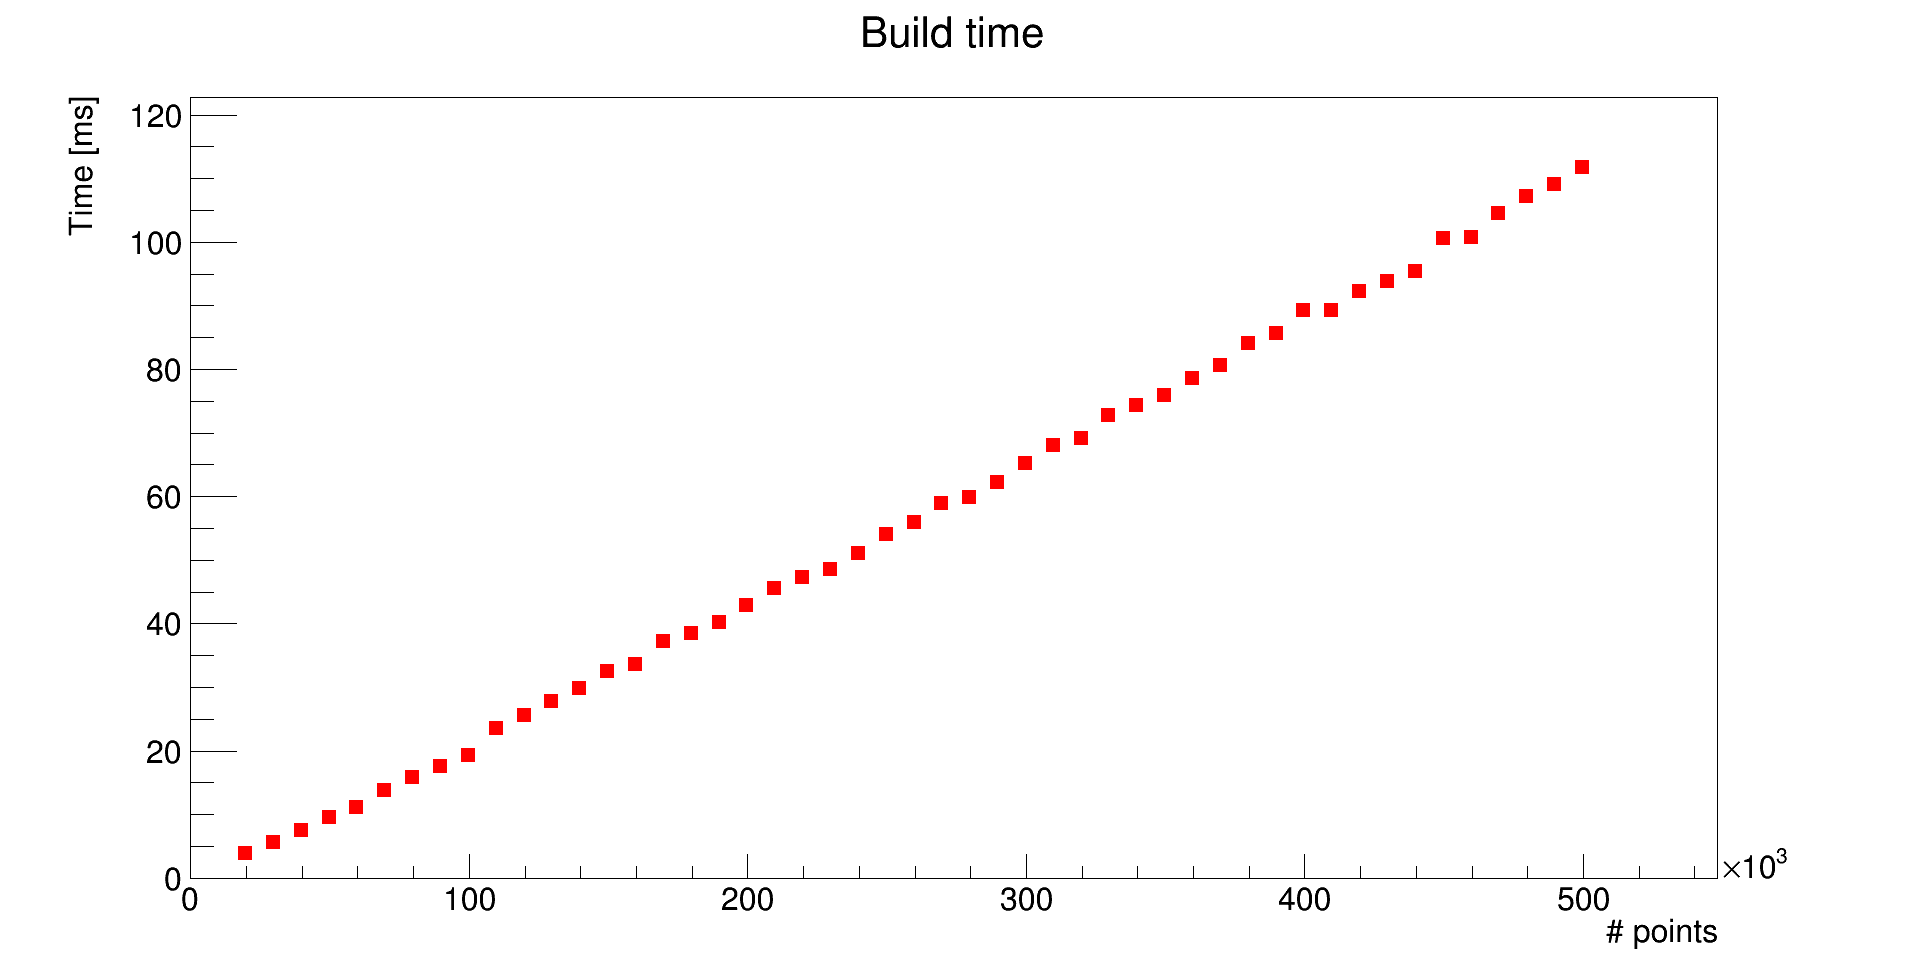
\includegraphics[scale=0.2]{images/fkdBuildTimes.png}
\end{center}
\end{changemargin}
\end{frame}

\begin{frame}{CUDA streams performance gain}
Relative performance gain for different number of CUDA streams:\\
\begin{changemargin}{-1cm}{-1cm}
\begin{center}
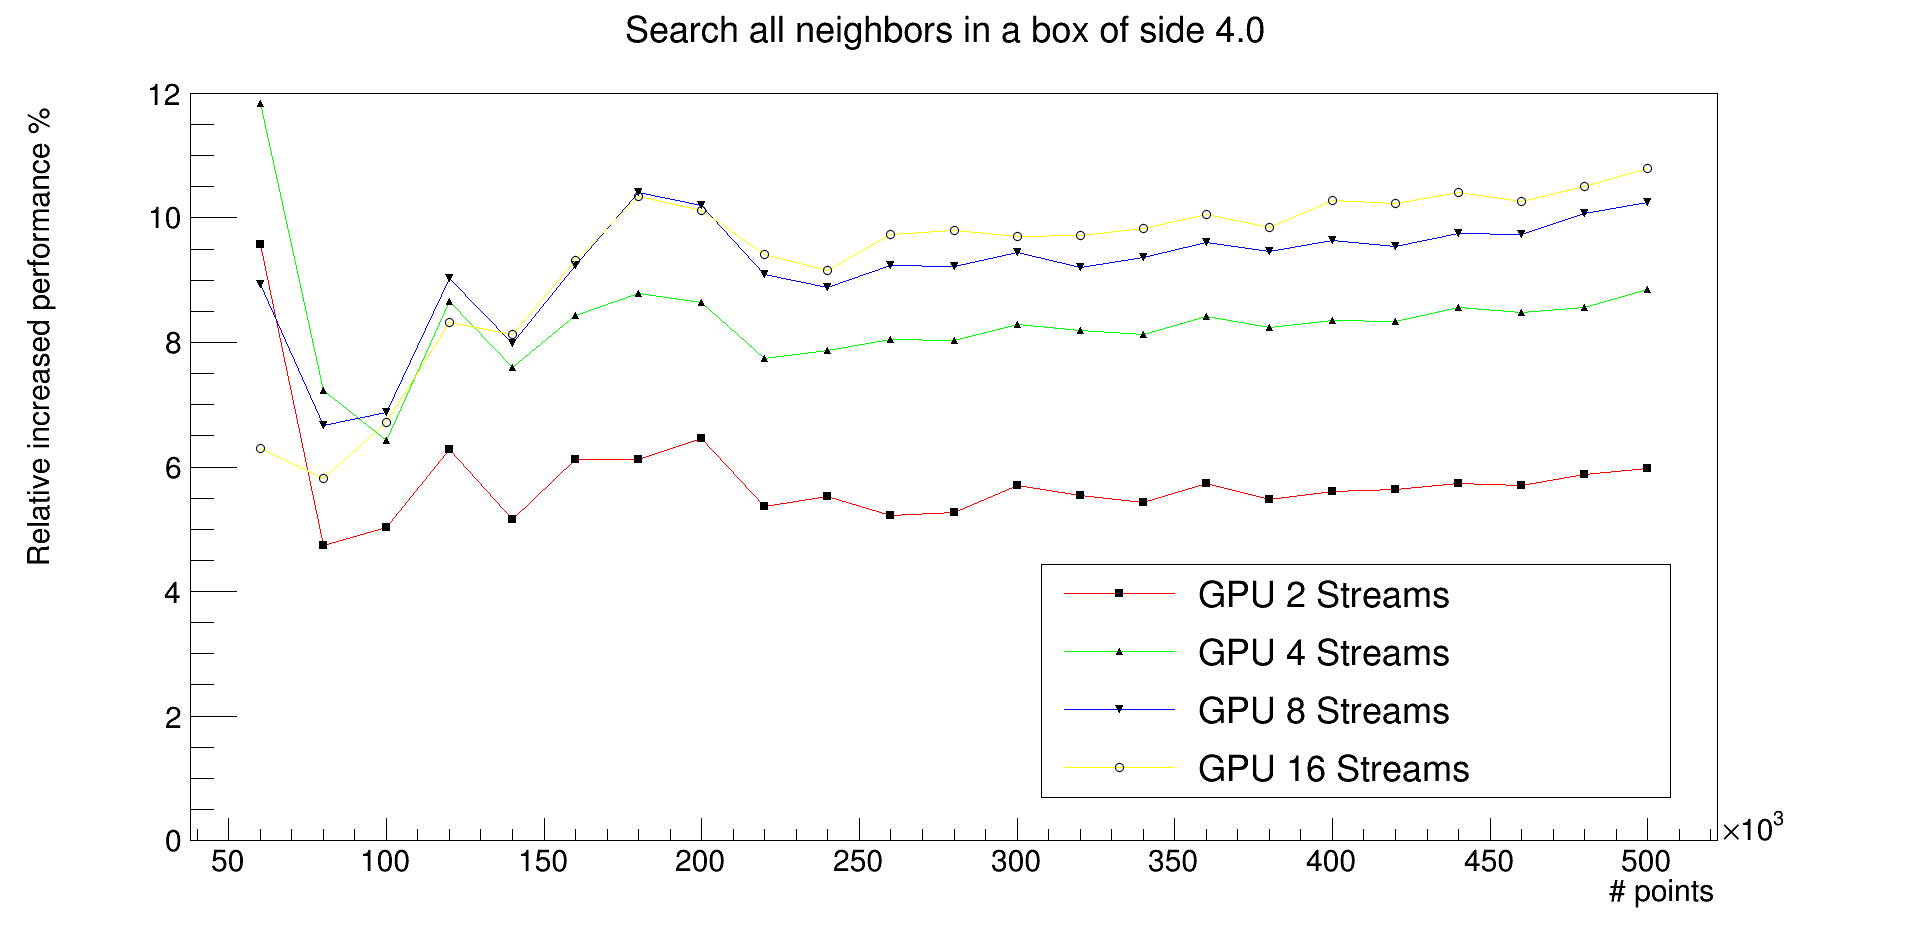
\includegraphics[scale=0.19]{images/fkdStreams.png}
\end{center}
\end{changemargin}
\end{frame}

\begin{frame}{Search times}
\begin{changemargin}{-1cm}{-1cm}
\begin{center}
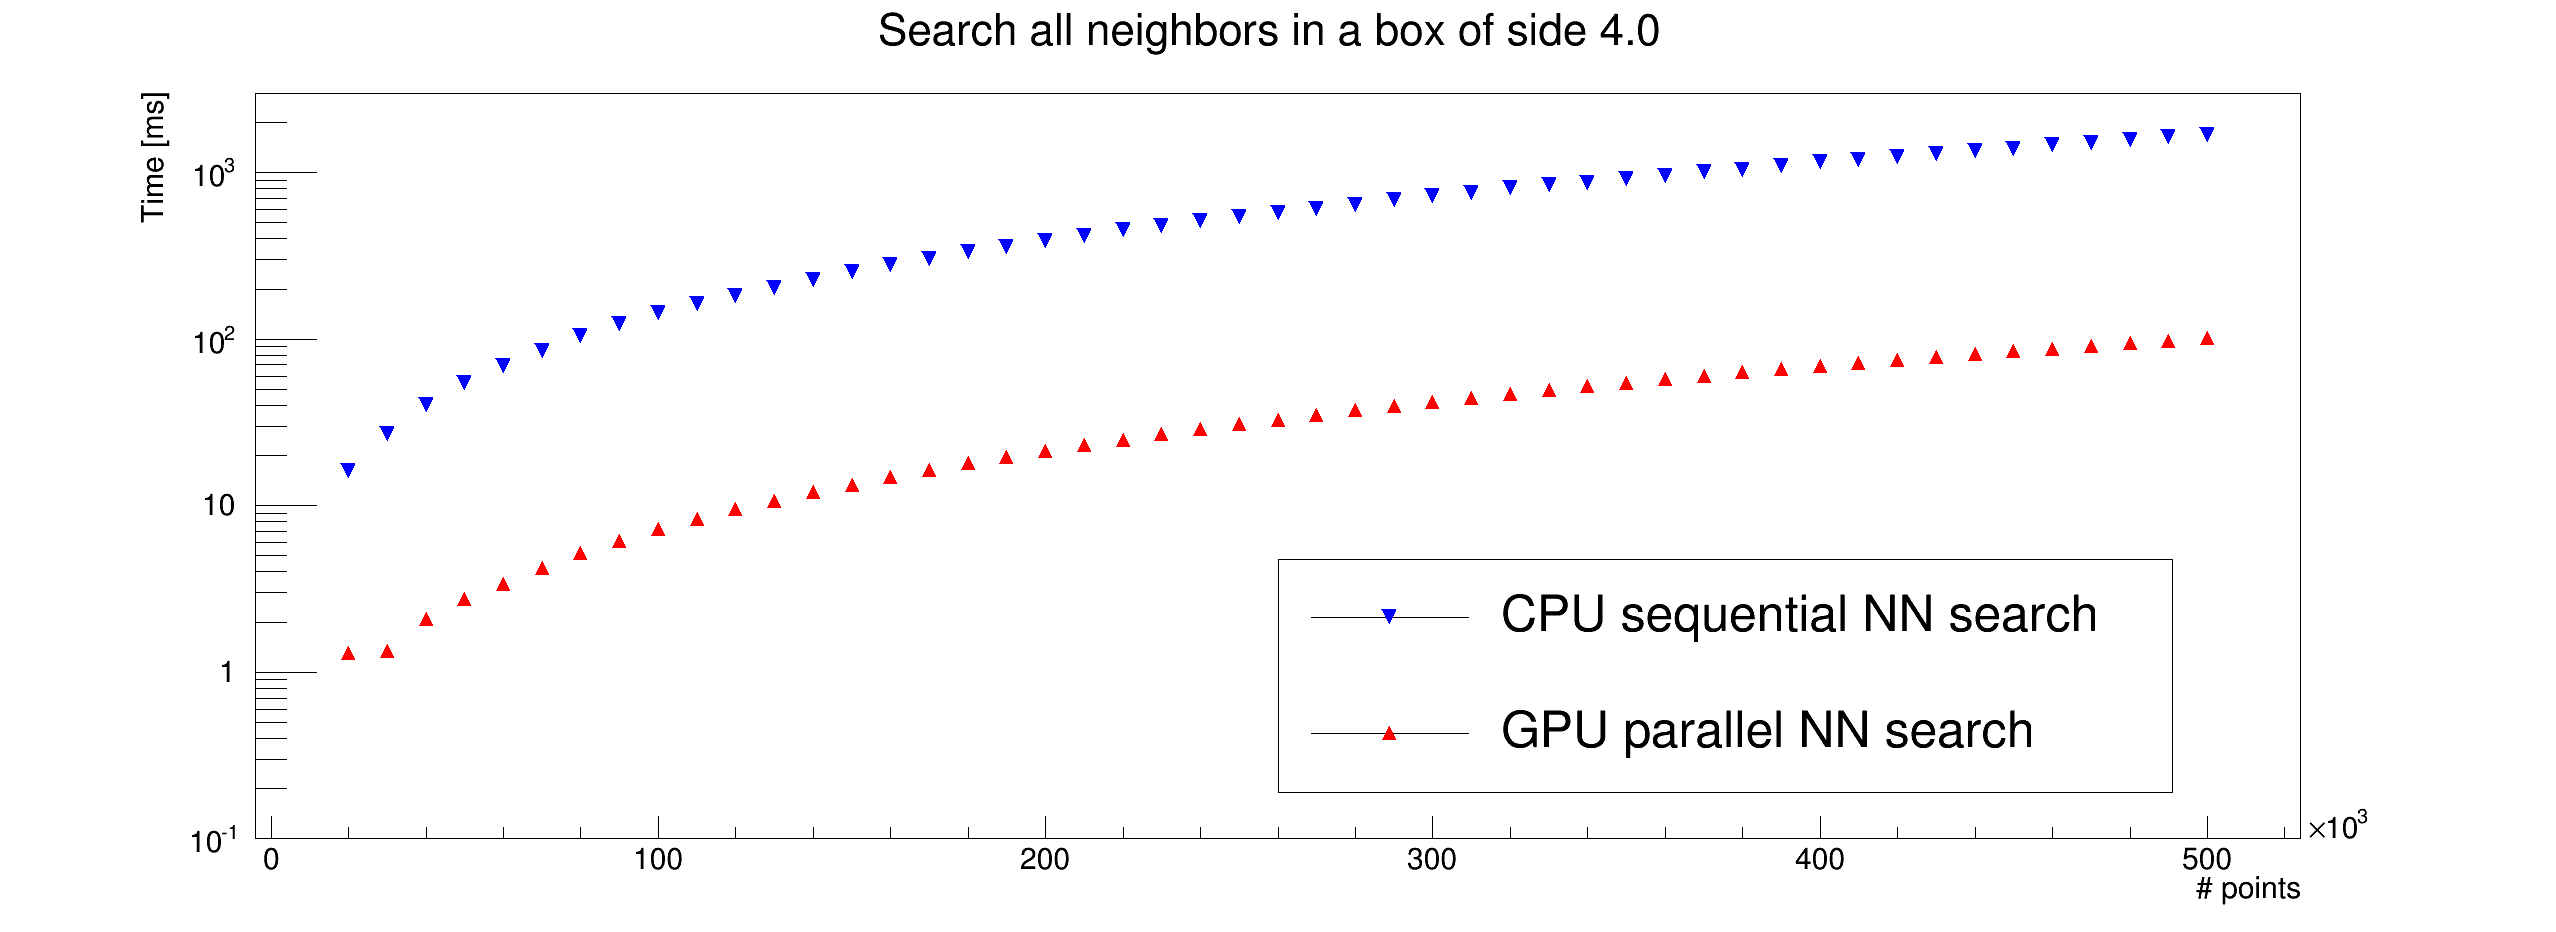
\includegraphics[scale=0.15]{images/fkdSearchTimes.png}
\end{center}
\begin{table}[h]
\begin{tabular}{ c || r r r r r r r r r r }
Points ($10^{3}$) & 50 & 100 & 150 & 200 & 250 & 300 & 350 & 400 & 450 & 500 \\
\hline
CPU ($\unit{ms}$) & 54 & 142 & 253 & 384 & 539 & 714 & 907 & 1143 & 1384 & 1682 \\
GPU ($\unit{ms}$) & 3 & 7 & 13 & 21 & 31 & 42 & 54 & 68 & 84 & 101 \\
\end{tabular}
\end{table}
\end{changemargin}
\end{frame}

\begin{frame}{Speedup}
\begin{changemargin}{-2cm}{-2cm}
\begin{center}
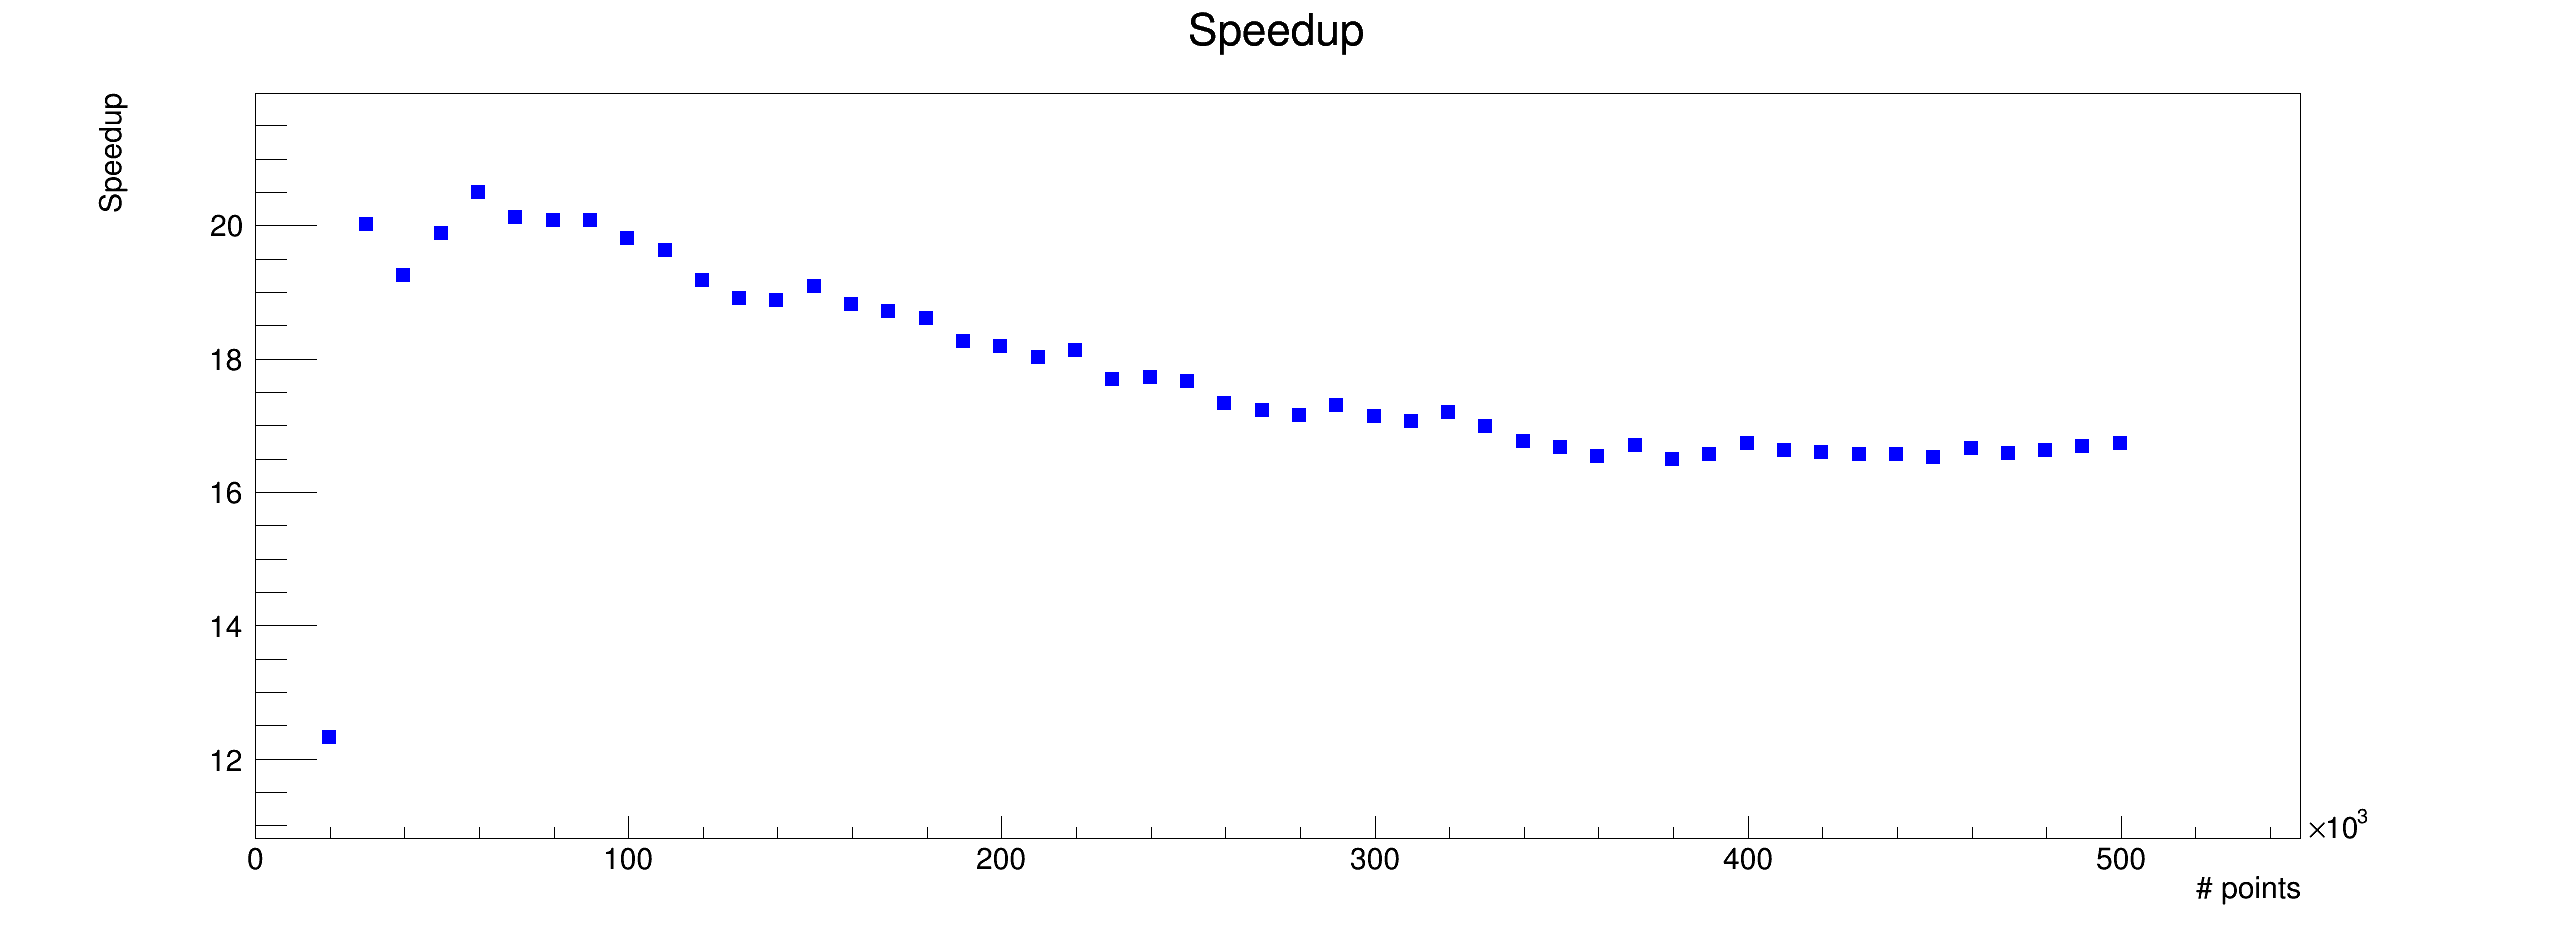
\includegraphics[scale=0.15]{images/fkdSpeedup.png}
\end{center}
\end{changemargin}
\vspace{5mm}
Speedup between \textbf{$\sim$16} and \textbf{$\sim$20}
\end{frame}

\begin{frame}{Fixed MAX NN Speedup}
Setting the maximum number of NN to \textbf{273} for all generated number of points results in a different speedup trend.
\vspace{10mm}
\begin{changemargin}{-2cm}{-2cm}
\begin{center}
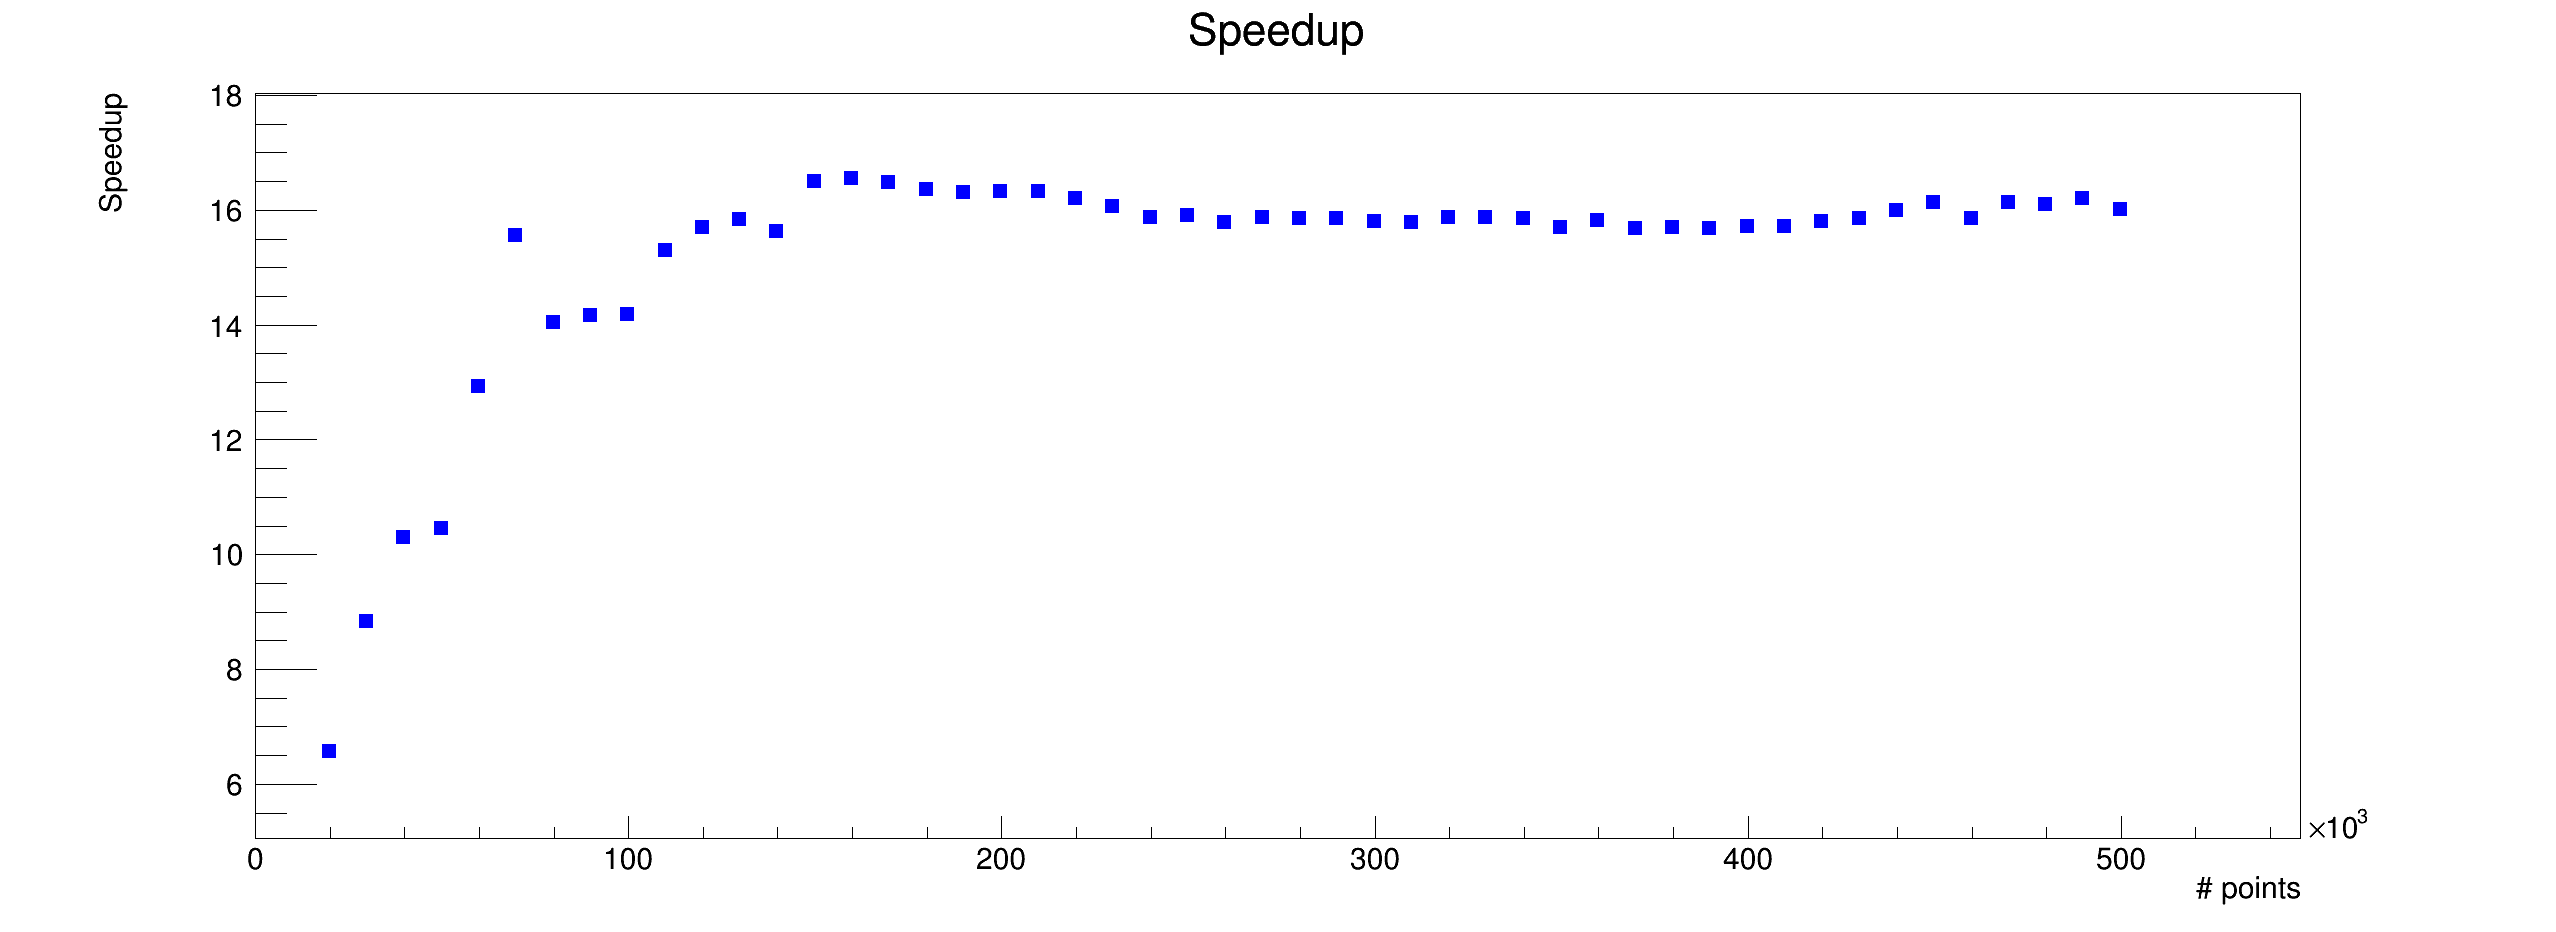
\includegraphics[scale=0.15]{images/200fkdSpeedup.png}
\end{center}
\end{changemargin}
\end{frame}

\begin{frame}{A HGCAL simulation}
10 sets of 10 events, 100 electrons, $P_t$:[10, 100]GeV/c, $\eta$ [1.6, 2.9]\\
\vspace{5mm}
\begin{changemargin}{-2cm}{-2cm}
\begin{center}
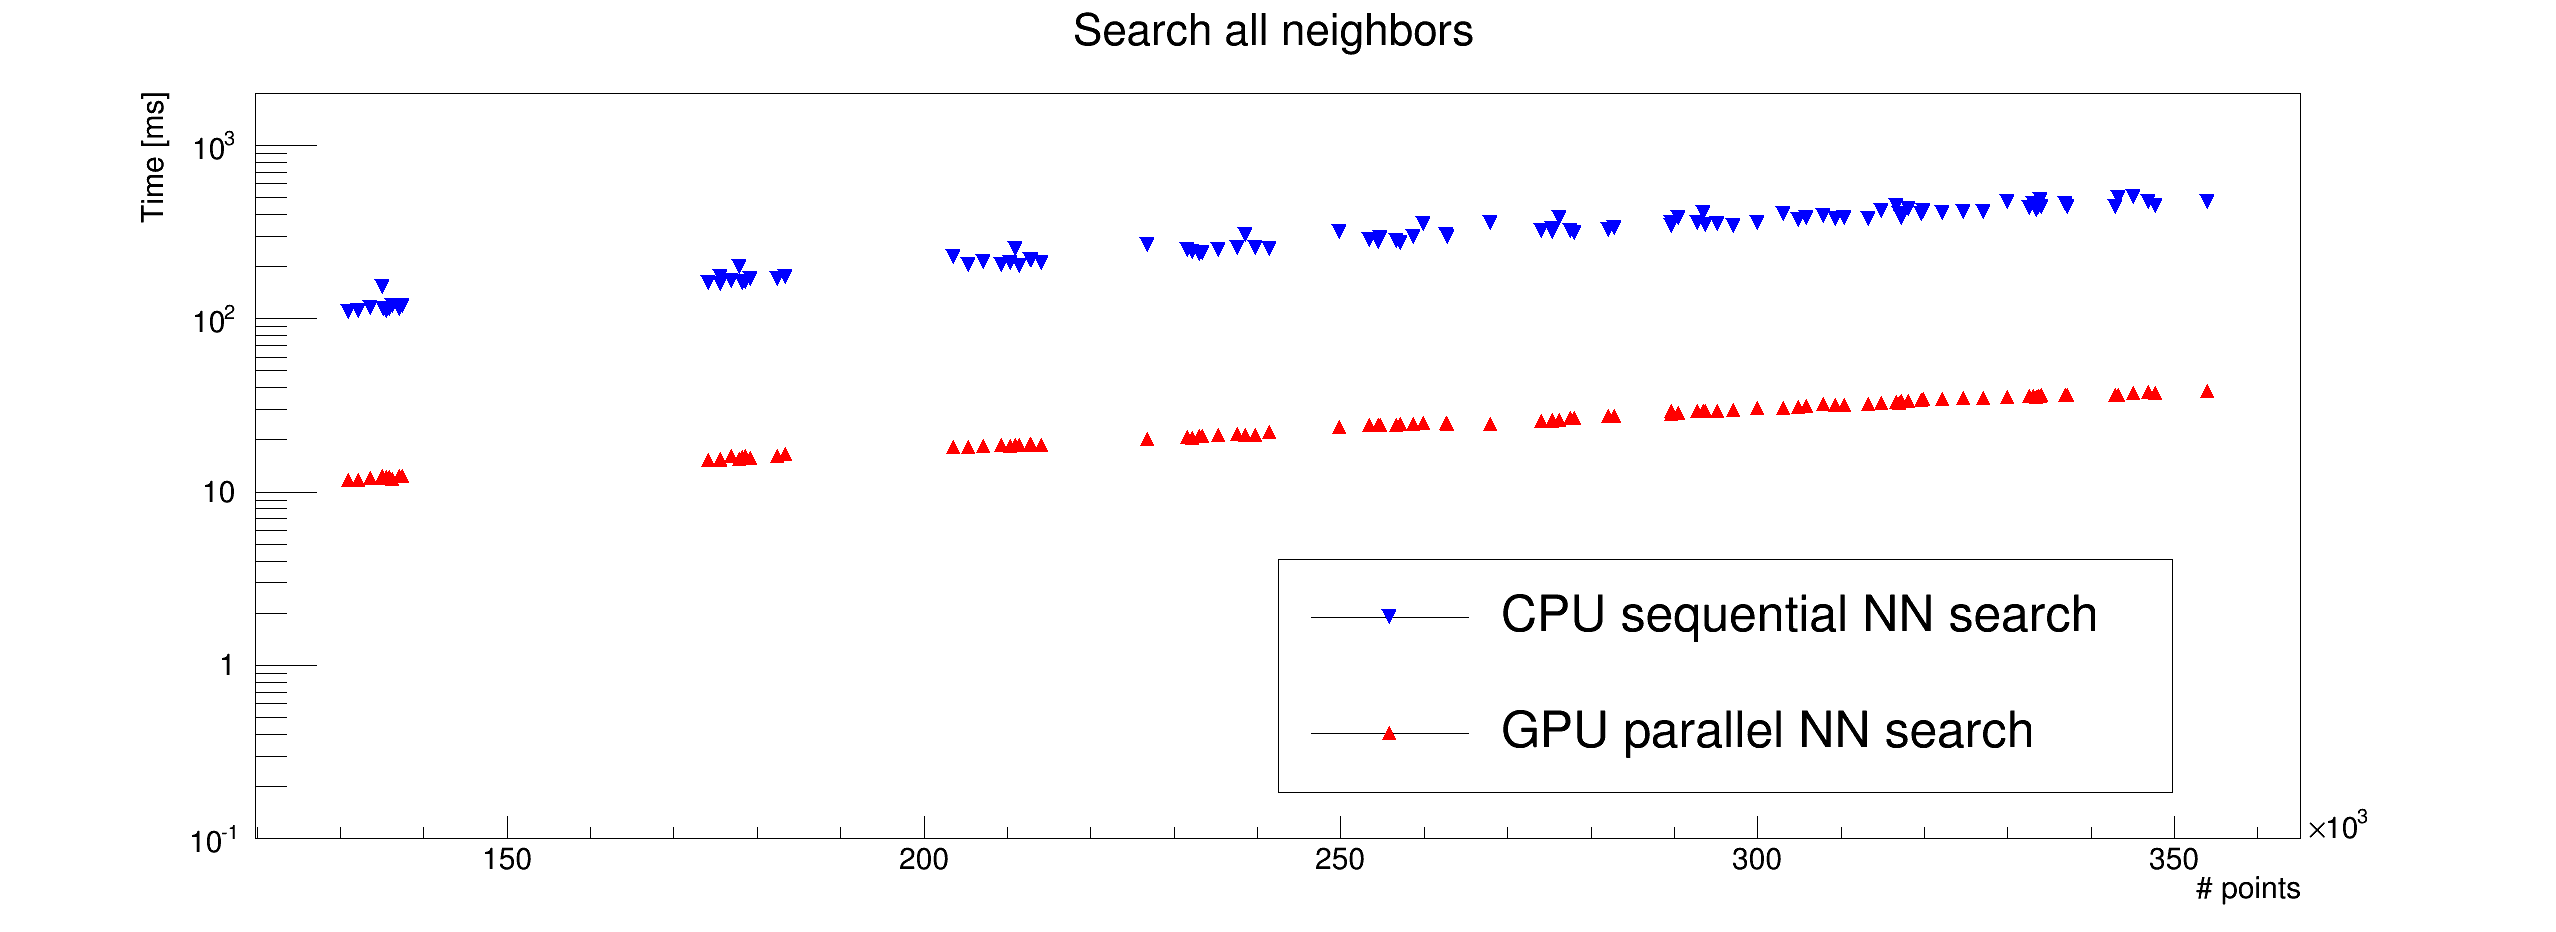
\includegraphics[scale=0.15]{images/RechitsSearchTimes.png}\\
\begin{table}[h]
\begin{tabular}{ c || r r r r r r r r r r}
Points ($10^{3}$) & 135 & 177 & 210 & 238 & 259 & 276 & 293 & 316 & 333 & 345 \\
\hline
CPU ($\unit{ms}$) & 152 & 199 & 251 & 302 & 349 & 378 & 405 & 444 & 482 & 503 \\
GPU ($\unit{ms}$) & 13 & 16 & 19 & 21 & 25 & 26 & 29 & 33 & 35 & 37 \\
\end{tabular}
\end{table}
\end{center}
\end{changemargin}
\end{frame}

\begin{frame}{HGCAL simulation speedup}
\begin{changemargin}{-2cm}{-2cm}
\begin{center}
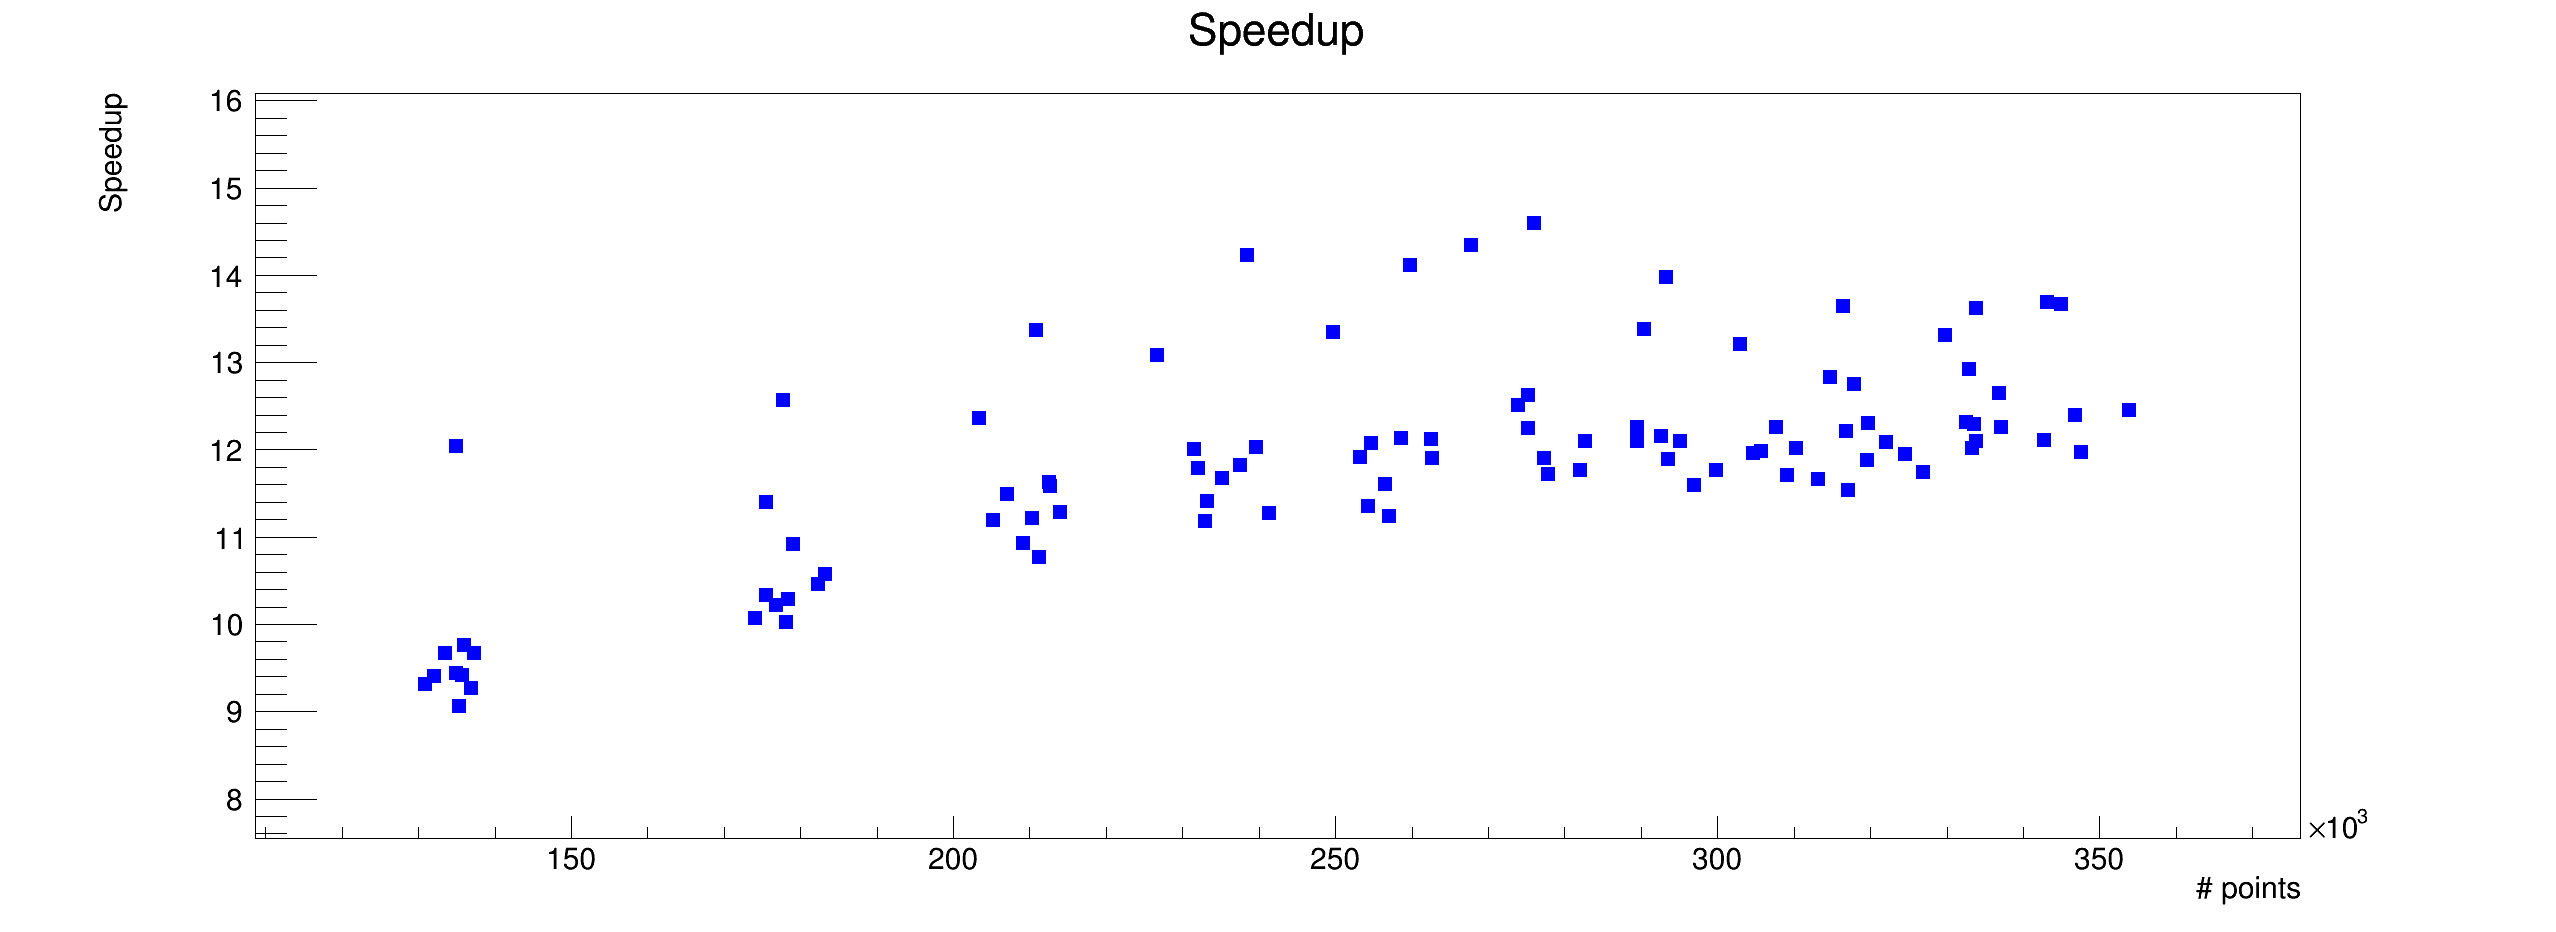
\includegraphics[scale=0.15]{images/RechitsSpeedup.png}
\end{center}
\end{changemargin}
\vspace{5mm}
Speedup between \textbf{$\sim$9} and \textbf{$\sim$15}
\end{frame}

\begin{frame}{New algorithm assessment}
Very promising performance:
\begin{itemize}
\item Build time acceptable: under 80 $\unit{ms}$ for 350000 points
\vspace{3mm}
\item Excellent search times: $\sim 500 \unit{ms}$ CPU and $\sim 37 \unit{ms}$ GPU
\vspace{3mm}
\item Speedup in line with Amdahl predictions
\end{itemize}
\vspace{5mm}
One sensible point:
\begin{itemize}
\item Performance highly affected by the maximum number\\ of NN considered
\end{itemize}
\end{frame}

\section{Energy consumption}

\begin{frame}{Energy consumption}
Two important reasons to design energy efficient software:
\begin{itemize}
\item Avoid energy waste
\item Limit heat dissipation
\item Save money
\end{itemize}
\vspace{5mm}
Methodology:
\begin{itemize}
\item Repeat the All NN search over $5 \times 10^5$ points several times
\item Measure the average power used
\item Measure the total time employed
\end{itemize}
\vspace{1mm}
Result: Avg. Power (W) X Total Time (s) / Search repetition $\rightarrow$\\
\vspace{2mm}
\begin{center}
J/search
\end{center}
\end{frame}

\begin{frame}{Instrumentation}
Two testing platforms:
\begin{itemize}
\item Workstation PC: Intel i7 CPU and Nvidia Tesla k40C GPU
\item Nvidia Tegra K1 SoC: ARM CPU and Nvidia Kepler GPU
\end{itemize}
\begin{center}
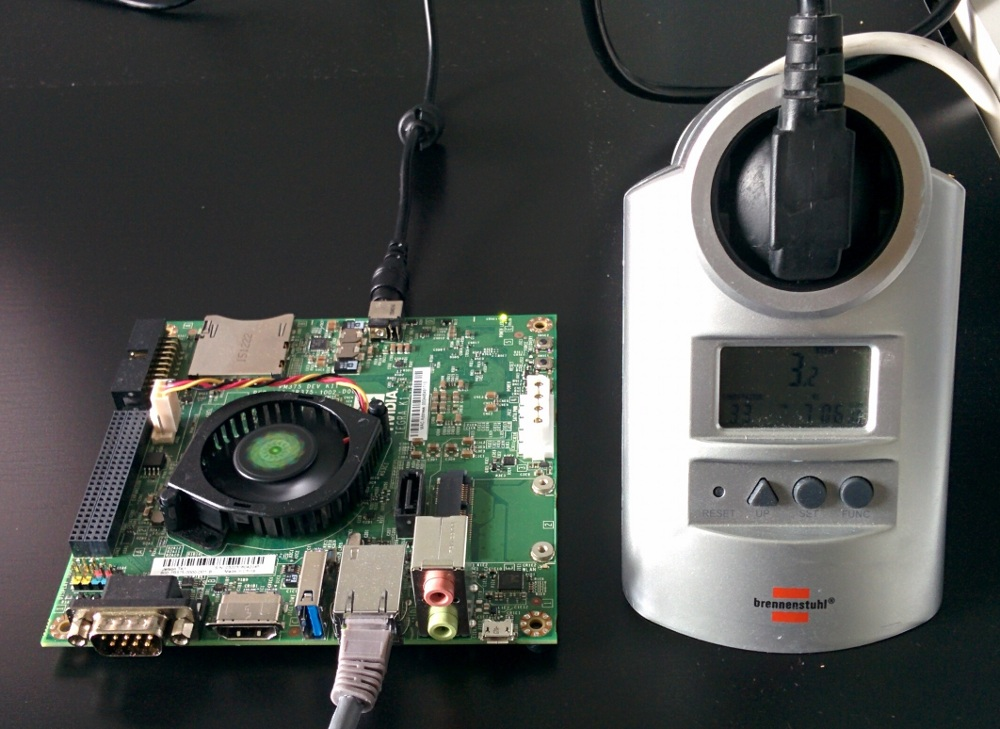
\includegraphics[scale=0.2]{images/tk1.jpg}\\
Power measurement: Power appliance meter and software
\end{center}
\end{frame}

\begin{frame}{Energy consumption measurements}
Workstation:
\vspace{2mm}
\begin{changemargin}{-2cm}{-2cm}
\begin{table}[h]
\begin{tabular}{c | l l l | l}
 & Power meter (W) & Software (W) & Timing (s) & Energy (J/search) \\
\hline
CPU & 52 $\pm$ 1 W & N.A. & 1.69 $\pm$ 0.01 s & 88 $\pm$ 2 J/search \\
GPU & 136 $\pm$ 1W & 135 $\pm$ 1 W & 97 $\pm$ 1 ms & 13 $\pm$ 1 J/search\\
\end{tabular}
\end{table}
\end{changemargin}
\vspace{10mm}
Tegra K1:
\vspace{2mm}
\begin{changemargin}{-2cm}{-2cm}
\begin{table}[h]
\begin{tabular}{c | l l | l}
 & Power meter (W) & Timing (s) & Energy (J/search) \\
\hline
CPU & 6.4 $\pm$ 0.1 W & 34.2 $\pm$ 0.1 s & 219 $\pm$ 3 J/search \\
GPU & 9.4 $\pm$ 0.1 W & 1.2 $\pm$ 0.1 s & 11 $\pm$ 1 J/search\\
\end{tabular}
\end{table}
\end{changemargin}
\end{frame}

\section{Conclusions}

\begin{frame}{Conclusions}
\begin{center}
\begin{itemize}
\item HGCAL will record up to 300k hits per event\\ during Phase-II
\vspace{3mm}
\item Event reconstruction (clusterization)\\ is computationally intensive
\vspace{3mm}
\item By 2023 hardware will have much better performance
\vspace{3mm}
\item Many-cores paradigm will probably stay
\vspace{3mm}
\item Massive parallelization non-trivial
\vspace{3mm}
\item Benefits extend to energy consumption
\end{itemize}
\end{center}
\end{frame}

\end{document}